\documentclass[12pt]{article}

\usepackage[utf8]{inputenc}
\usepackage[english]{babel}

\usepackage{amsmath}

\usepackage{mathtools}

\usepackage{amssymb}

\usepackage{stmaryrd}

\usepackage{amsthm}

\usepackage{latexsym}

\usepackage{IEEEtrantools}

\usepackage{eucal}

\usepackage{bbm}

\usepackage[dvipsnames]{xcolor}


\usepackage{bussproofs}

\usepackage{graphicx}
\graphicspath{ {./images/} }

\usepackage{stmaryrd}


\usepackage{tikz}

\usetikzlibrary{arrows}



\usepackage{tikz-cd}



%\usepackage{tikzit}

%\input{sample.tikzstyles} Add styles doc here

%\input{sample.tikzdefs}

\usepackage[normalem]{ulem}

\usepackage{hyperref}

\usepackage[dvipsnames]{xcolor}

\definecolor{darkgreen}{RGB}{35, 89, 52}

\hypersetup{
	colorlinks=true,
	linkcolor=darkgreen,
	filecolor=magenta,      
	urlcolor=MidnightBlue,
	citecolor=darkgreen,
	pdftitle={Linear Logic and Resources Notebook},
	bookmarks=true
}

\title{Linear Logic and Co-Design Notebook}

\author{Marius Furter}

\date{\today}

\usepackage[
backend=bibtex,
style=alphabetic,
citestyle=alphabetic]{biblatex}
\addbibresource{LLCD.bib}

\theoremstyle{definition}

\newtheorem{definition}{Definition}[section]



\theoremstyle{plain} 

\newtheorem{lemma}{Lemma}[section]



\theoremstyle{plain} 

\newtheorem{proposition}{Proposition}[section]



\theoremstyle{plain}

\newtheorem{theorem}{Theorem}[section]


\theoremstyle{plain}

\newtheorem{question}{Question}[section]


\theoremstyle{remark}

\newtheorem{example}{Example}[section]

\newtheorem*{excont}{Example \continuation}
\newcommand{\continuation}{??}
\newenvironment{continueexample}[1]
{\renewcommand{\continuation}{\ref{#1}}\excont[continued]}
{\endexcont}


\theoremstyle{remark}

\newtheorem{remark}{Remark}[section]

\newcommand{\zuz}[1]{%

	\begin{tikzpicture}[#1]%

	\draw[semithick, line cap = round, line join = round] (-0.3ex,0.35ex) -- (0.5ex,0.35ex);

	\draw[semithick, line cap = round, line join = round] (0.5ex,0.35ex) -- (0.5ex,-0.5ex);

	\draw[semithick, line cap = round, line join = round] (0.5ex,-0.5ex) -- (1.5ex,-0.5ex);

	\draw[semithick, line cap = round, line join = round] (0,0) -- (1ex,0);%

	\draw[semithick, line cap = round, line join = round] (1ex,0) -- (1ex,-0.85ex);

	\draw[semithick, line cap = round, line join = round] (1ex,-0.85ex) -- (1.8ex,-0.85ex);

	\end{tikzpicture}%

} 



\renewcommand\qedsymbol{\zuz{scale=1.5}}

\newcommand{\mc}[1]{\mathcal{#1}}

\newcommand{\sub}{\subseteq}

\newcommand{\Hom}{\text{Hom}}

\newcommand{\im}{\text{im}}

\newcommand{\id}{\text{id}}

\makeatletter
\def\slashedarrowfill@#1#2#3#4#5{%
	$\m@th\thickmuskip0mu\medmuskip\thickmuskip\thinmuskip\thickmuskip
	\relax#5#1\mkern-7mu%
	\cleaders\hbox{$#5\mkern-2mu#2\mkern-2mu$}\hfill
	\mathclap{#3}\mathclap{#2}%
	\cleaders\hbox{$#5\mkern-2mu#2\mkern-2mu$}\hfill
	\mkern-7mu#4$%
}
\def\rightslashedarrowfill@{%
	\slashedarrowfill@\relbar\relbar\mapstochar\rightarrow}
\newcommand\xslashedrightarrow[2][]{%
	\ext@arrow 0055{\rightslashedarrowfill@}{#1}{#2}}
\makeatother


\begin{document}

\maketitle
\tableofcontents

\section{Categories in Linear Logic}

\subsection{The Category of Derivations}

Given a sequent calculus $S$, we form the category of derivations in $S$, denoted $\mathbf{Der}_S$ as follows. The objects are well-formed sequents 
$$\Gamma, A \vdash B \qquad \Gamma \vdash A \multimap B \qquad \ldots$$  
and the morphisms are valid derivations based on the rules of $S$, for example,

\begin{prooftree}
\AxiomC{$\Gamma, A \vdash B$}
\RightLabel{\scriptsize($\multimap$ Right)}
\UnaryInfC{$\Gamma \vdash A \multimap B$}
\end{prooftree}
Composition is given by the composition of derivations. 
\begin{center}
	

	\AxiomC{$\Gamma \vdash B$}
	\RightLabel{\scriptsize(weakening Left)}
	\UnaryInfC{$\Gamma, A \vdash B$}
	\noLine
	\UnaryInfC{}
	\noLine
	\UnaryInfC{$\Gamma, A \vdash B$}
	\RightLabel{\scriptsize($\multimap$ Right)}
	\UnaryInfC{$\Gamma \vdash A \multimap B$}
	\DisplayProof
\qquad $\rightsquigarrow$ \qquad
	\AxiomC{$\Gamma \vdash B$}
	\RightLabel{\scriptsize(weakening Left)}
	\UnaryInfC{$\Gamma, A \vdash B$}
	\RightLabel{\scriptsize($\multimap$ Right)}
	\UnaryInfC{$\Gamma \vdash A \multimap B$}
	\DisplayProof

\end{center}
It is clearly associative and has the ``do nothing'' sequent
\begin{prooftree}
	\AxiomC{$\Gamma \vdash \Delta$}
	\RightLabel{\scriptsize(identity)}
	\UnaryInfC{$\Gamma \vdash \Delta$}

\end{prooftree}
as identity.

This all works fine for unary rules. To accommodate rules of higher arity, we need to allow multiple sources for our morphisms. We could then think of $\mathbf{Der}_S$ as a multicategory (colored operad) or, alternatively, replace objects by lists of objects and introduce a monoidal product $\boxplus$ that allows us to concatenate these lists. The unit for this monoidal product is the empty list $[\;]$. We shall write lists of objects $[A,B,C]$ as $A \boxplus B \boxplus C$, that is we omit the brackets for lists of length one. For now, due to a current lack a familiarity with multicategories, we shall regard $\mathbf{Der}_S$ as a monoidal category. In this setting, rules of higher arity become morphisms from lists of length greater 1 to lists of length 1. For example, the cut rule
\begin{prooftree}
	\AxiomC{$\Gamma, A \vdash B$}
	\AxiomC{$\Delta, B \vdash C$}
	\RightLabel{\scriptsize(Cut)}
	\BinaryInfC{$\Gamma, \Delta, A \vdash C$}
\end{prooftree}
is a morphism $(\Gamma, A \vdash B) \boxplus (\Delta, B \vdash C) \rightarrow \Gamma, \Delta, A \vdash C$. The axiom
\begin{prooftree}
	\AxiomC{}
		\RightLabel{\scriptsize(Axiom)}
	\UnaryInfC{$A \vdash A$}
\end{prooftree}
is a morphism $[\;] \rightarrow A \vdash A$.

We may now view the category $\mathbf{Der}_S$ as being generated by the rules of the sequent calculus $S$: We fix some set of propositions $\Gamma,\Delta,\Lambda, \ldots$ and consider all sequents that can be formed from these. We then form all finite lists of such sequents and add morphisms according to the rules of $S$. Finally $\mathbf{Der}_S$ is obtained by closing this structure under composition.

\begin{question}
	Read about operads / multicategories in Leinster's book Chapter 2. Think about the algebras of $\mathbf{Der}_S$.
\end{question}

\subsection{The Category of Propositions}

The category of proposition $\mathbf{Prop}_S$ has a objects propositions $\Gamma,\Delta,\Lambda, \ldots$ and as morphisms proofs of sequents $\Gamma \vdash \Delta$. The compostion of morphisms is given by the cut rule
\begin{prooftree}
	\AxiomC{$A \vdash B$}
	\AxiomC{$B \vdash C$}
	\RightLabel{\scriptsize(Cut)}
	\BinaryInfC{$A \vdash C$}
\end{prooftree}
which turn two proofs into one. We note that cut rule depends on the sequent calculus. For example, in intuitionistic linear logic it is
\begin{prooftree}
	\AxiomC{$\Gamma \vdash A$}
	\AxiomC{$\gamma_1, A, \gamma_2 \vdash B$}
	\RightLabel{\scriptsize(Cut)}
	\BinaryInfC{$\gamma_1, \Gamma, \gamma_2 \vdash B$}
\end{prooftree} 
Our basic rule is obtained with empty contexts $\gamma_1,\gamma_2$.

\subsection{The Relation between Der and Prop}

To start with suppose that our calculus $S$ consists only of unary rules. In this case $\mathbf{Der}_S$ is simply a category with a special object for the empty sequent $[\;]$. We observe that the arrows of $\mathbf{Prop}_S$ are special derivations: An arrow $\Gamma \rightarrow \Delta$ in $\mathbf{Prop}_S$ corresponds to an arrow in $\mathbf{Der}_S$ of the form $[\;] \rightarrow \Gamma \vdash \Delta$. Therefore $\mathbf{Prop}_S(\Gamma,\Delta) \cong \mathbf{Der}_S([\;],\Gamma \vdash \Delta)$. Moreover, each element of $\mathbf{Der}_S(\Gamma \vdash \Delta, A \vdash B)$ gives a function $\mathbf{Prop}_S(\Gamma,\Delta) \rightarrow \mathbf{Prop}_S(A,B)$, obtained by composing derivations. This yields a functor $F: \mathbf{Der}_S \rightarrow \mathbf{Set}$ mapping objects $(\Gamma \vdash \Delta) \mapsto \mathbf{Prop}_S(\Gamma,\Delta)$ and derivations $\Gamma,\Delta \rightarrow A,B$ to the induced function $\mathbf{Prop}_S(\Gamma,\Delta) \rightarrow \mathbf{Prop}_S(A,B)$. Indeed, functoriality is immediate.

We extend the construction above to the case where $S$ has rules of arbitrary arity. In this case the objects in $\mathbf{Der}_S$ are lists of sequents. Because $\boxplus^n [\;] \cong [\;]$ we still have the correspondence $\mathbf{Prop}_S(\Gamma,\Delta) \cong \mathbf{Der}_S([\;],\Gamma \vdash \Delta)$. Next we note that if we have an arrow $d: A_1 \boxplus \ldots \boxplus A_n \rightarrow B_1 \boxplus \ldots \boxplus B_m$ then $n \geq m$ because the rules of $S$ are many to one. Moreover, we can regard $d$ as consisting of $m$ parallel derivations $d_i: A_{i_1} \boxplus \ldots \boxplus A_{i_r} \rightarrow B_i$. Writing $A_{i_j} = \Gamma_{i_j} \vdash \Delta_{i_j}$ and $B_i = \Psi_i \vdash \Omega_i$, we see that each $d_i$ induces a function
$$\mathbf{Prop}_S(\Gamma_{i_1},\Delta_{i_1}) \times \ldots \times  \mathbf{Prop}_S(\Gamma_{i_r},\Delta_{i_r}) \rightarrow \mathbf{Prop}_S(\Psi_i, \Omega_i).$$
Hence $d$ induces a function
$$\prod_i \mathbf{Prop}_S(\Gamma_{i_1},\Delta_{i_1}) \times \ldots \times  \mathbf{Prop}_S(\Gamma_{i_r},\Delta_{i_r}) \rightarrow \prod_i \mathbf{Prop}_S(\Psi_i, \Omega_i).$$

We now face the problem that the decomposition of the $A_i$ is not the same for every derivation with the same source and target as $d$. However, writing $A_j = \Gamma_{j} \vdash \Delta_{j}$, we have a natural iso
$$\prod_i \mathbf{Prop}_S(\Gamma_{i_1},\Delta_{i_1}) \times \ldots \times  \mathbf{Prop}_S(\Gamma_{i_r},\Delta_{i_r}) \cong \prod_{j=1}^n \mathbf{Prop}_S(\Gamma_{j},\Delta_{j})$$
by reordering the big product. This suggests that we assign a list of sequents $(\Gamma_{1} \vdash \Delta_{1}) \boxplus \ldots \boxplus (\Gamma_{n} \vdash \Delta_{n})$ to the product $\prod_{j=1}^n \mathbf{Prop}_S(\Gamma_{j},\Delta_{j})$. A morphism 
$$f: (\Gamma_{1} \vdash \Delta_{1}) \boxplus \ldots \boxplus (\Gamma_{n} \vdash \Delta_{n}) \rightarrow (\Psi_{1} \vdash \Omega_{1}) \boxplus \ldots \boxplus (\Psi_{m} \vdash \Omega_{m})$$
is then assigned to the function
$$\tilde f: \prod_{j=1}^n \mathbf{Prop}_S(\Gamma_{j},\Delta_{j}) \rightarrow \prod_i \mathbf{Prop}_S(\Psi_i, \Omega_i)$$
which it induces by the procedure described above, possibly composing with the reordering isomorphism. 

Explicitly, we can describe $\tilde f$ as follows: Given a tuple of proofs of sequents $$ (\Gamma_{1} \vdash \Delta_{1}, \ldots, \Gamma_{n} \vdash \Delta_{n}), $$ regard them as a derivation $$[\;] \rightarrow (\Gamma_{1} \vdash \Delta_{1}) \boxplus \ldots \boxplus (\Gamma_{n} \vdash \Delta_{n})$$ and compose with $f$ to get a derivation $$[\:] \rightarrow  (\Psi_{1} \vdash \Omega_{1}) \boxplus \ldots \boxplus (\Psi_{m} \vdash \Omega_{m})$$ which corresponds to a tuple of proofs of sequents $$(\Psi_1 \vdash \Omega_{1}, \ldots, \Psi_{m} \vdash \Omega_{m}).$$ The functoriality of this assignment is again immediate. Hence, we also get a functor $F: \mathbf{Der}_S \rightarrow \mathbf{Set}$ in the case of a general sequent calculus $S$. Furthermore, $F$ maps monoidal products in $\mathbf{Der}_S$ to cartesian products in $\mathbf{Set}$. We have $F([\;]) = \{*\}$ by definition, which aligns with the intuition that there is exactly one trivial proof of the empty sequent. Therefore $F$ is a strict monoidal functor into $(\mathbf{Set},\times,\{*\})$.

\begin{question}
	Regarding $\mathbf{Der}_S$ as an operad, can we describe the above as an operad algebra?
\end{question}

We conclude by observing that for $A_i = \Gamma_{i} \vdash \Delta_{i}$ we have 
$$\mathbf{Der}_S([\;],A_1 \boxplus \ldots \boxplus A_n) \cong  \mathbf{Prop}_S(\Gamma_{1}, \Delta_{1}) \times \ldots \times \mathbf{Prop}_S(\Gamma_{n}, \Delta_{n}) = F(A_1 \boxplus \ldots \boxplus A_n)$$
so in fact $F$ is represented by $[\;]$. Furthermore, we have defined the way $F$ acts on arrows in terms of this isomorphism, so the isomorphism is natural. Hence $F \cong \Hom([\;], -)$. By Yoneda we have that for any element $x \in F(A)$ there is a unique morphism $f: [\;] \rightarrow A$ such that $F(f)(*) = x$. This is saying that proofs correspond precisely to derivations starting from $[\;]$.

\section{Linear Logic and Co-Design}

\subsection{Basic Definitions} \label{basic defs}

Let $\mc{R}$ and $\mc{F}$ be posets. $\mc{R}$ represents resources and $\mc{F}$ represents functionalities. For $a,b \in \mc{R}$, we interpret $a \leq b$ as meaning ``if I have $a$, then I also have $b$''. For example, $2\$ \leq 1\$$. This is the opposite convention that is currently in use, but better suits the Linear Logic interpretation. To avoid confusion, we write $a \rightarrow b$, or $a \vdash b$, instead of $a \leq b$. This also fits nicely with the fact that we will be regarding the posets as categories. 

In Co-Design we consider what functionalities we can obtain from given resources.
\begin{definition}[Feasibility Relation]
	Let $\mc{R}$, $\mc{F}$ be posets. A \emph{feasibility relation} $\mc{R} \xslashedrightarrow{} \mc{F}$ is a monotone map $\mc{R}^\text{op} \times \mc{F} \rightarrow \mathbf{Bool}$, where $\mathbf{Bool}$ denotes the poset generated by $\texttt{false} \rightarrow \texttt{true}$. If we regard posets as $\mathbf{Bool}$-categories, then feasibility relations are just $\mathbf{Bool}$-profunctors.
\end{definition}

\begin{remark}
	We can draw a feasibility relation $\mc{R} \xslashedrightarrow{} \mc{F}$ as an internal diagram:
	\begin{center}
		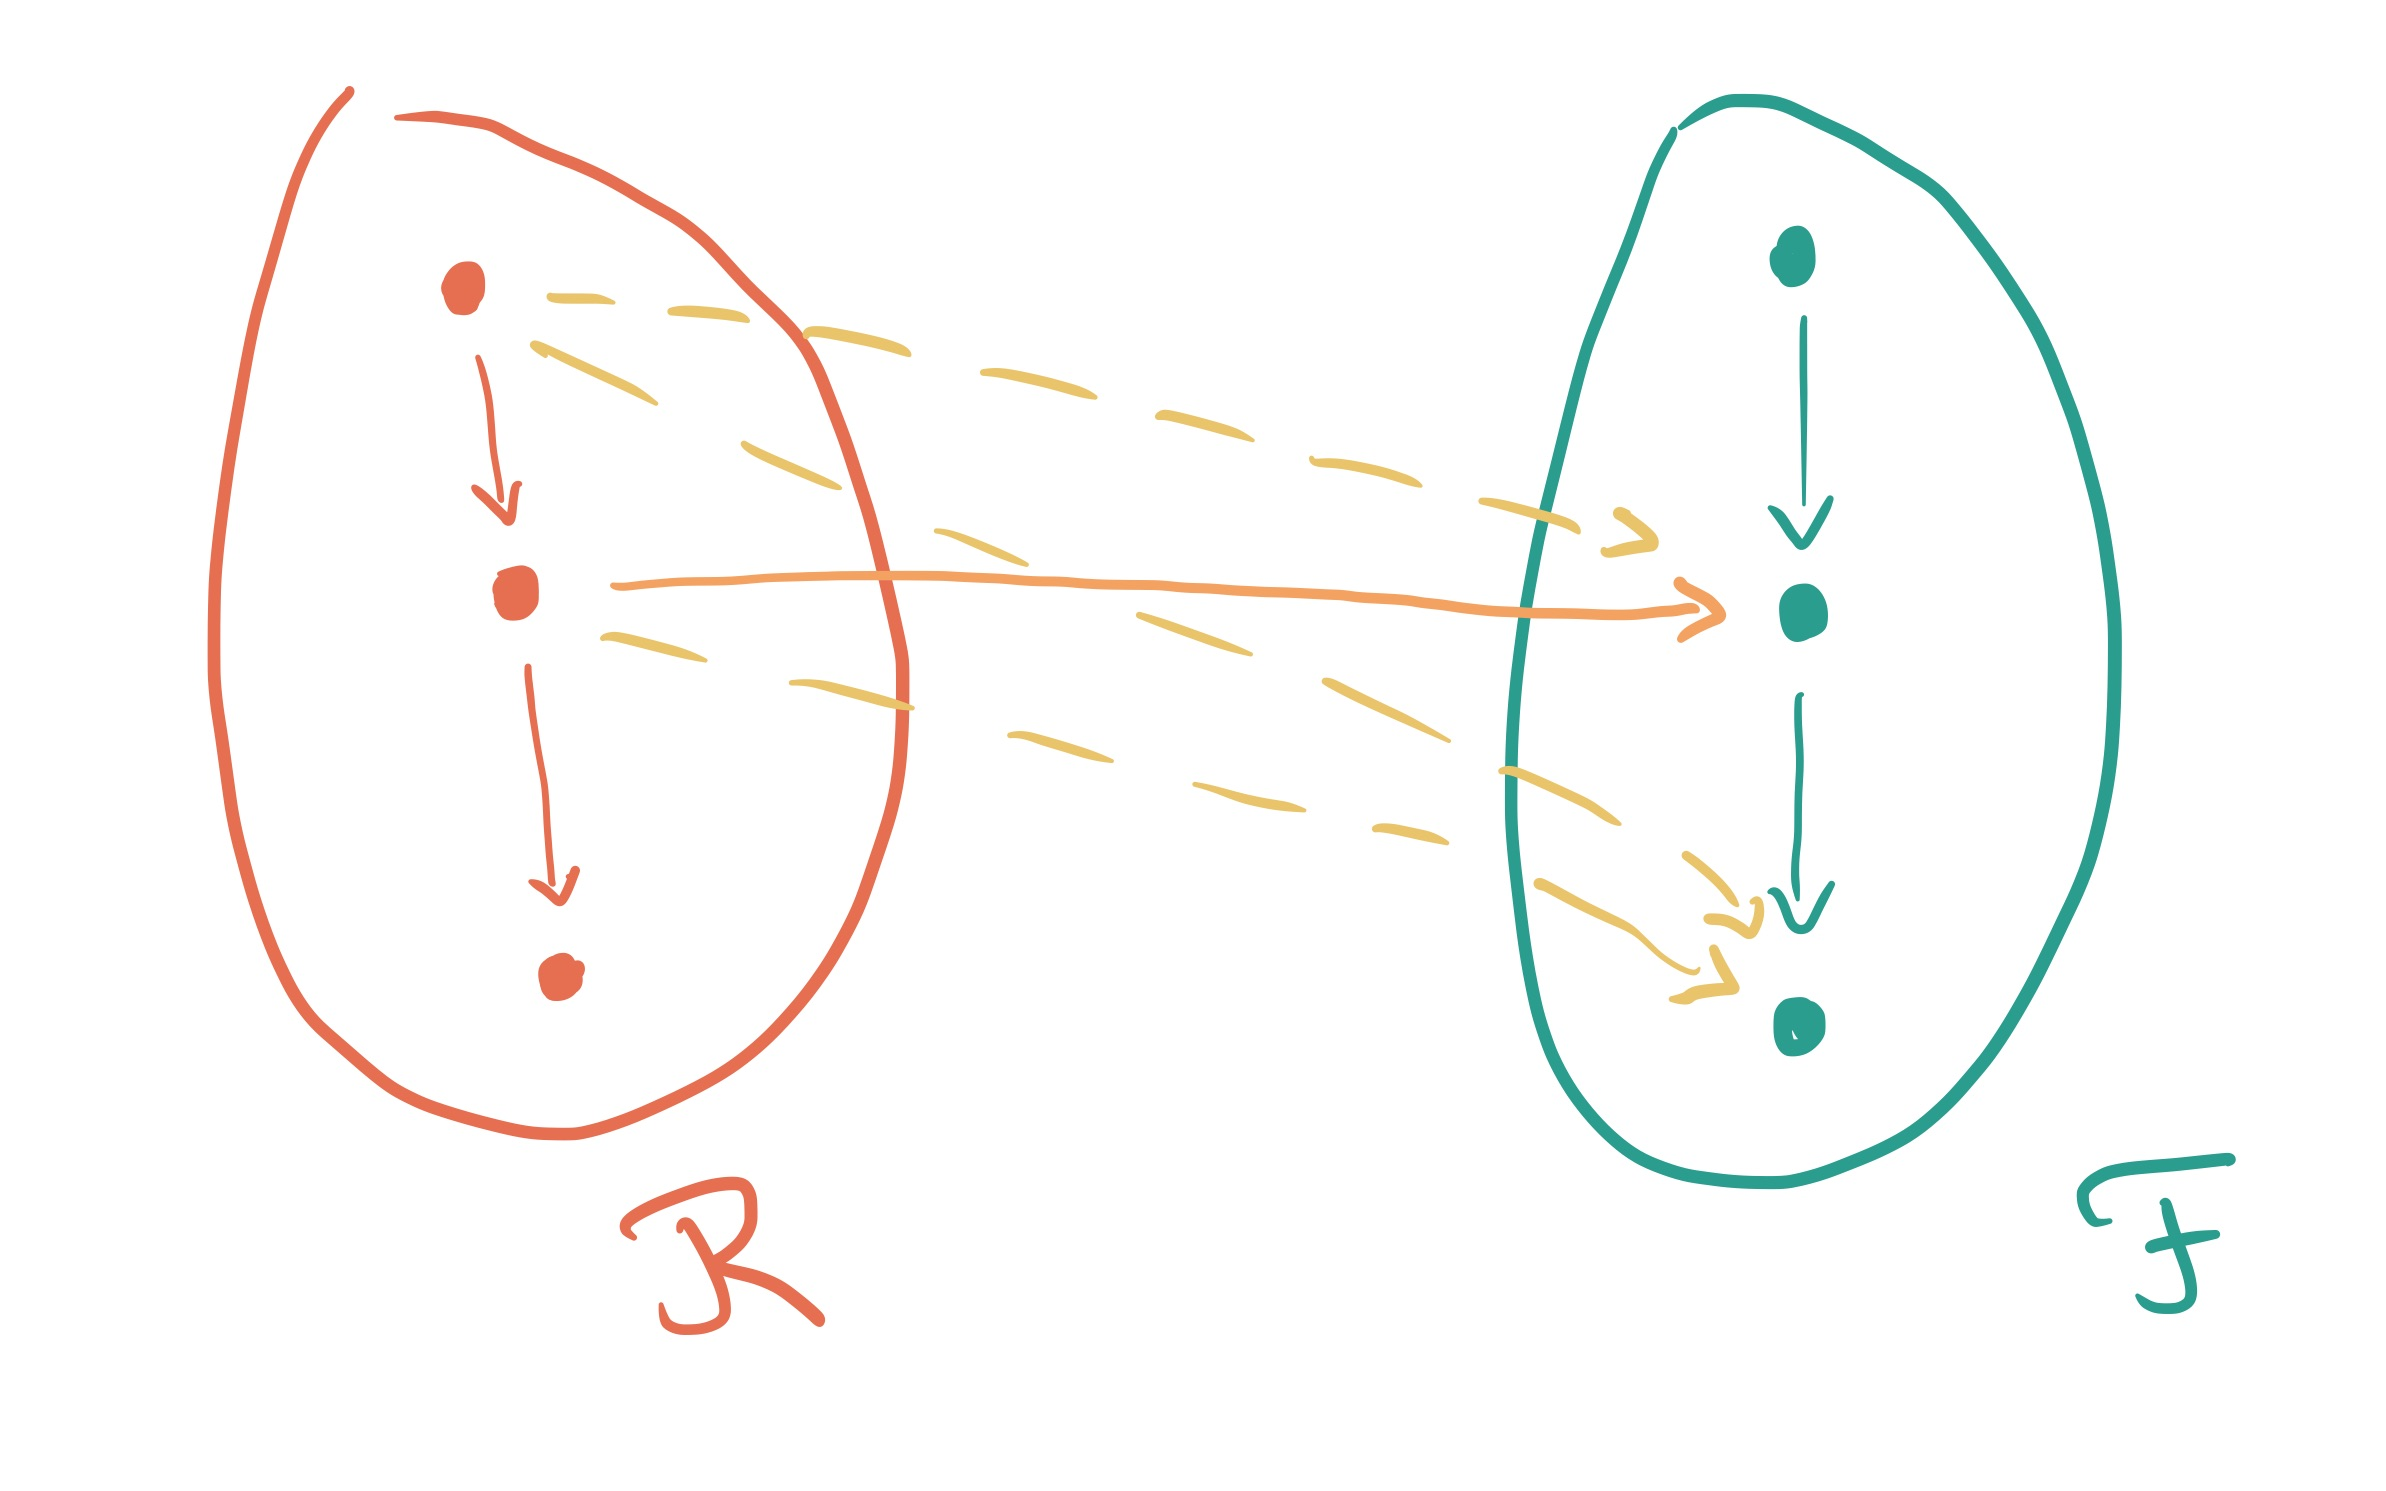
\includegraphics[width=\textwidth/2]{section2/feas_internal-1}
	\end{center}
	The orange and yellow arrows mean that a given pair is mapped to \texttt{true}. Absence of an arrow means the pair is mapped top \texttt{false}. Additionally, we may think of a feasibility relation as being generated by certain assignments. The solid orange arrow induces the dashed yellow arrows by composition with the arrows internal to both $\mc{R}$ and $\mc{F}$. 
\end{remark}

We can now define a category in which feasibility relations live.
\begin{definition}
	The category $\mathbf{DP}$ of co-design problems has posets as objects and feasibility relations as morphisms. Composition is given by profunctor compostition. Explicitly, if we have feasibility relations $\Phi: \mc{X} \xslashedrightarrow{} \mc{Y}$ and $\Psi: \mc{Y} \xslashedrightarrow{} \mc{Z}$, then
	$$ 
	\Phi \fatsemi \Psi (x,z) = \bigvee_{y \in \mc{Y}}(\Phi(x,y) \wedge \Psi(y,z)).
	$$
\end{definition}

Every feasibility relation  $\mc{R} \xslashedrightarrow{\Phi} \mc{F}$ naturally gives rise to two dual optimization problems. If we fix an $f \in \mc{F}$, then we can ask what the minimal set of resources $r \in \mc{R}$ are, such that $\Phi(r,f) = \texttt{true}$, that is $(r,f)$ is feasible. In formulae:
\begin{IEEEeqnarray*}{rCl}
	f_\text{max} & = & \text{Max} \{r \in \mc{R} \:\: |\: \Phi(r,f) = \texttt{true} \} \\ 
	& = &\{r \in \mc{R} \:\: |\: \Phi(r,f) = \texttt{true} \text{ and } \forall r': \Phi(r',f) = \mathtt{true} \wedge r \rightarrow r' \Rightarrow r=r' \}.
\end{IEEEeqnarray*}

Observe that the minimality condition implies that this set is an antichain in $\mc{R}$. Hence we get a function $h: \mc{F} \rightarrow \mathsf{A}\mc{R}$, $f \mapsto f_\text{max}$ where $\mathsf{A}\mc{R}$ denotes the set of antichains of $\mc{R}$. We can put a partial ordering on $\mathsf{A}\mc{R}$ by saying $A \leq B$ iff $\downarrow A \sub \: \downarrow B$, where $\downarrow$ denotes the lower closure operator. In our convention the lower closure of a set is all of the resources / functionalities that are `more expensive' than items in the set.

\begin{lemma}
	If all ascending chains in $\mc{R}$ are finite, then the map $h: \mc{F} \rightarrow \mathsf{A}\mc{R}$ is monotone. That is, if $f \rightarrow g$, then $\downarrow f_\text{max} \sub \: \downarrow g_\text{max}$.
\end{lemma}
\begin{proof}
	Let $f \rightarrow g$, and $x \in \: \downarrow f_\text{max}$. This means $x \rightarrow r$ for some $r \in f_\text{max}$. Because $\Phi(r,f) = \texttt{true}$ also $\Phi(x,g) = \texttt{true}$ using monotonicity in both arguments. Consider $\{s \in \mc{R} \:\: |\: x \rightarrow s  \text{ and } \Phi(s,g) = \texttt{true} \}$. This set is non-empty because it contains x itself. Moreover it has to contain a maximal element, otherwise we could build an infinite ascending chain. This maximum $m$ will be an element of $g_\text{max}$, hence we have an arrow $x \rightarrow m$, which means $x \in \downarrow g_\text{max}$
\end{proof}

\paragraph{Warning!} The map $h$ does not have to monotone in general (even if one uses upper closure or the opposite orderings). The ascending chain condition assures that one does not have arbitrarily cheap resources. To see that it is necessary consider $\mc{R} = (\mathbb{Z},\leq)$, $\mc{F} = {a \rightarrow b}$ with feasibility relation $\Psi(r,f) = \texttt{true}$ iff $f = b$ or $r \leq 0$. Then $a_\text{max} = \text{Max}\{n \in \mathbb{Z} | \Psi(r,a) = \texttt{true}\} = 0$ and $b_\text{max} = \text{Max}\{n \in \mathbb{Z} | \Psi(r,b) = \texttt{true}\} = \text{Max }\mathbb{Z} = \emptyset$. Hence $\downarrow a_\text{max} = \mathbb{Z}_{\leq 0} \nsubseteq \emptyset = \downarrow b_\text{max}$.

\subsection{Sites to Structure}

The main goal of this project is to add some of the structure of Linear Logic to the co-design framework. In principle, there are several places in the theory where one could consider implementing these concepts. Here we describe four possibilities and give some thoughts on how they may be related.
\begin{center}
	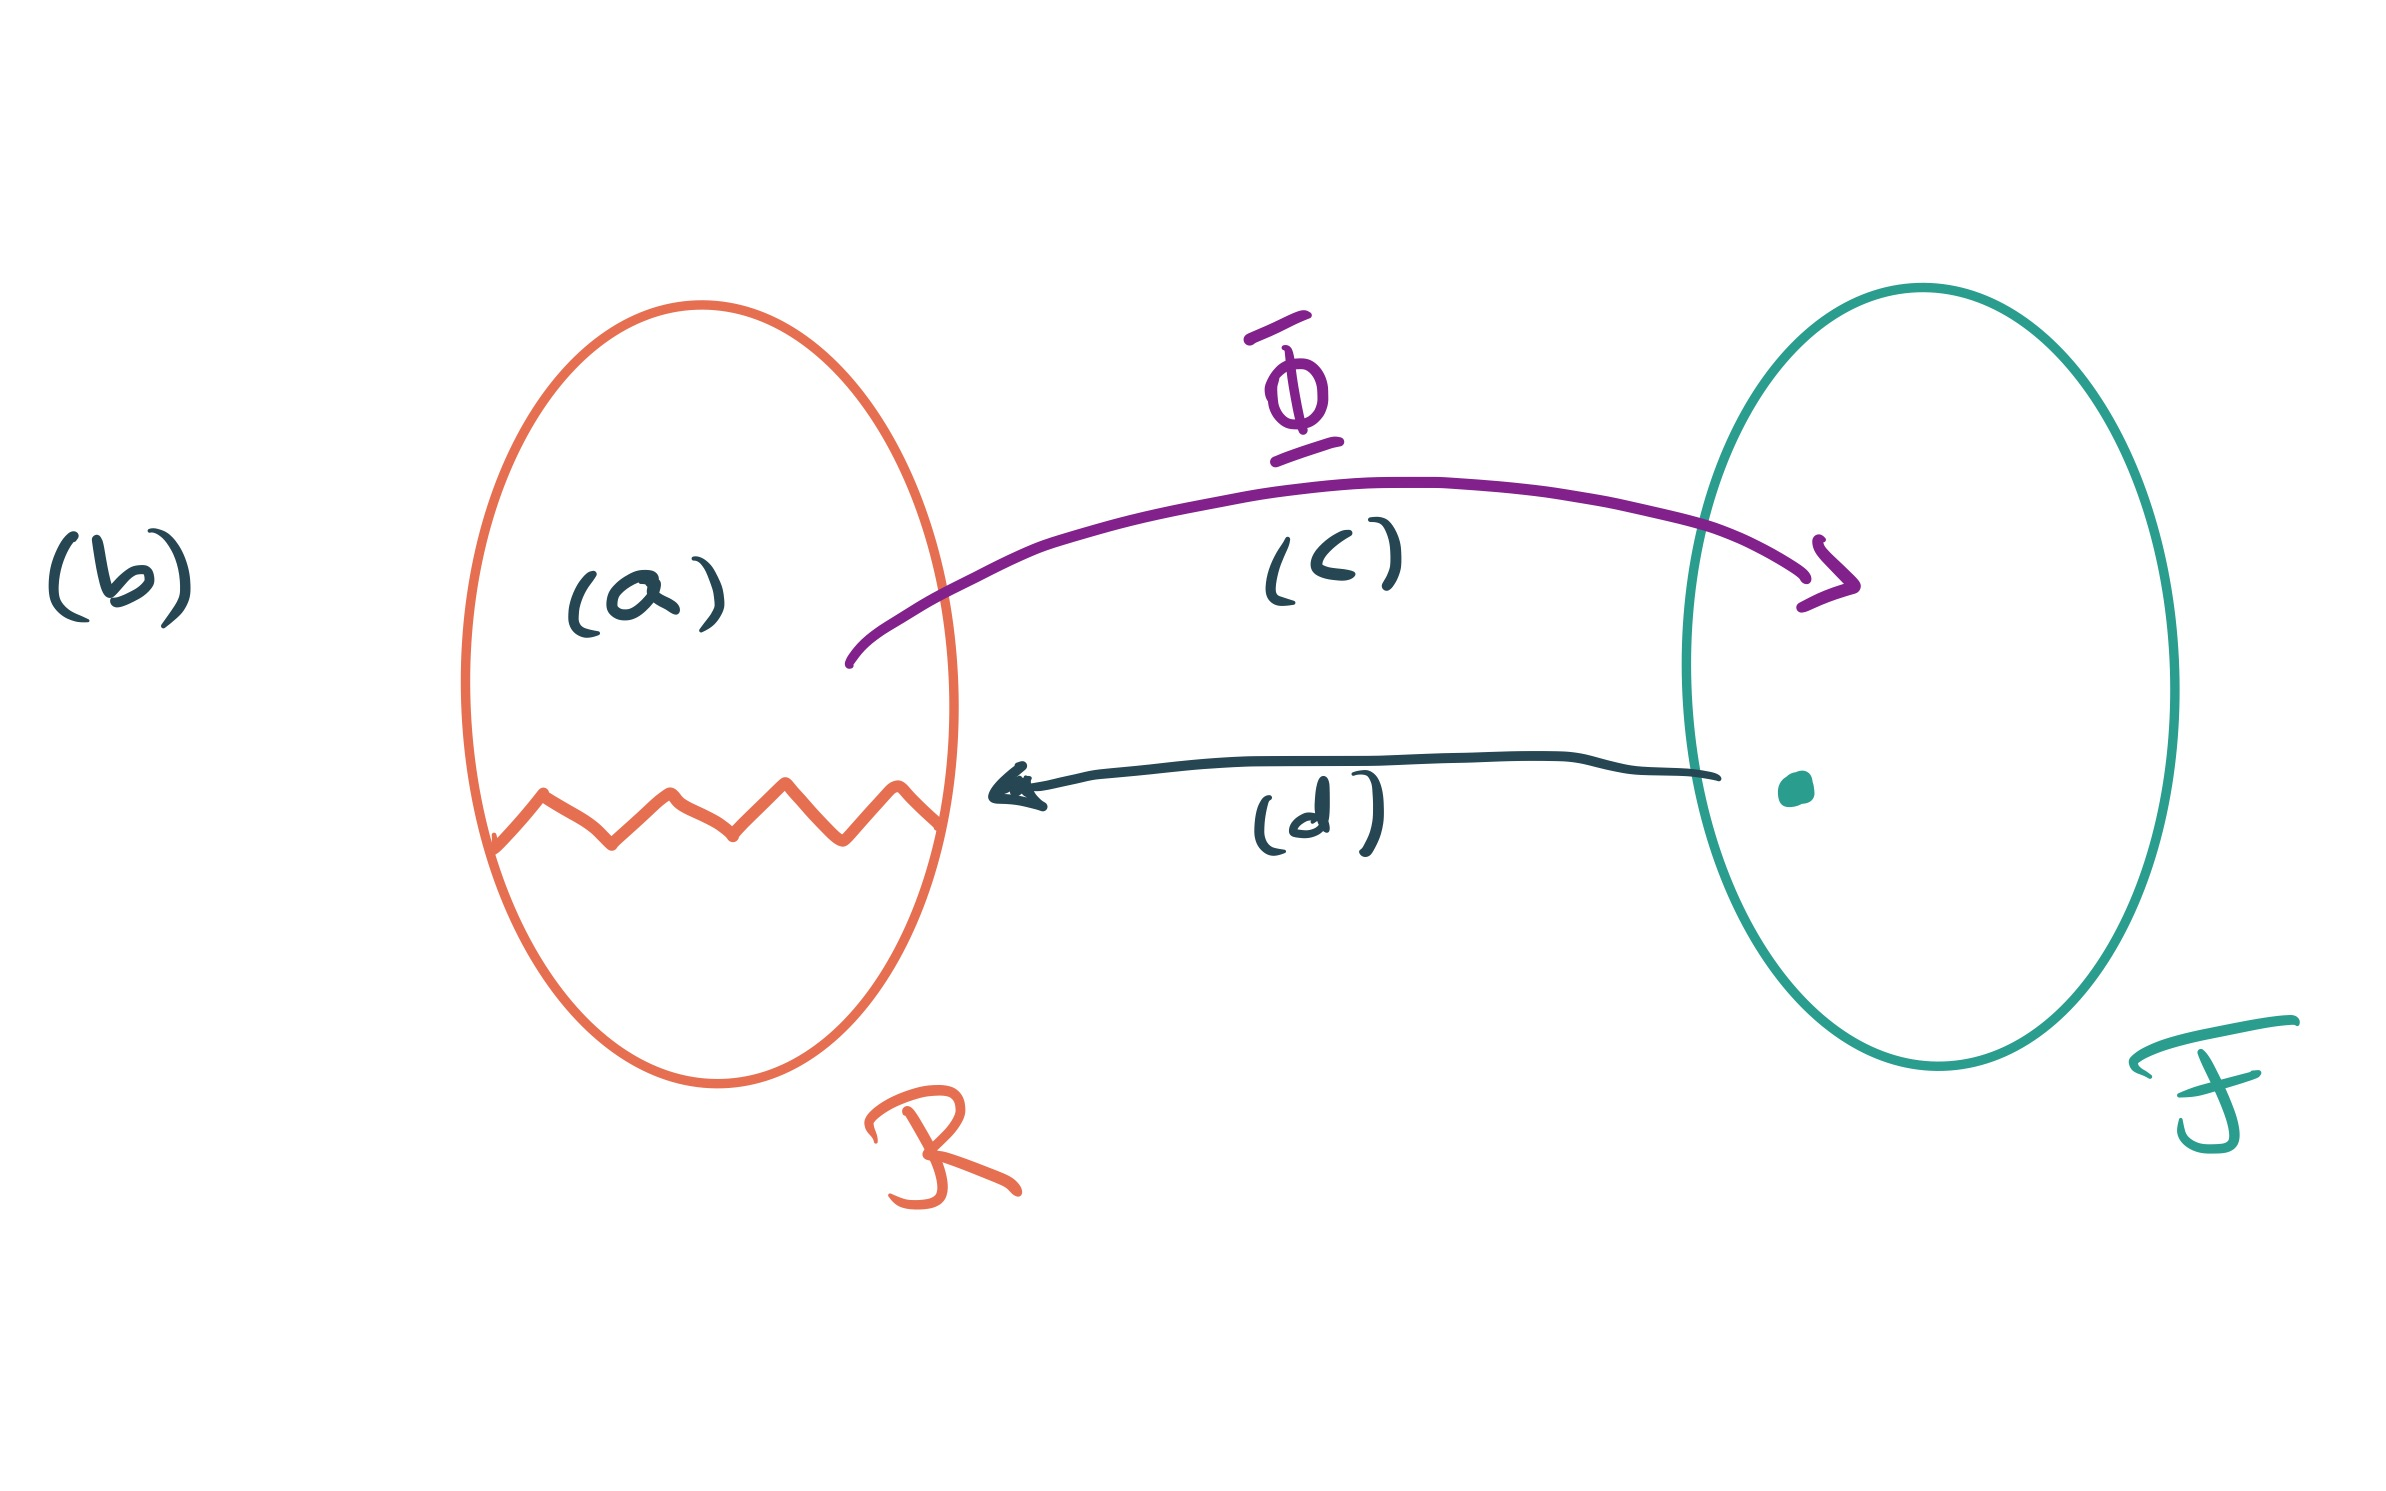
\includegraphics[width=250pt]{section2/sites_structure-1}
\end{center}

One can imagine having Linear Logic (LL) structure:
\begin{itemize}
	\item[(a)] internal to the resource / functionality posets. This would involve restricting the objects of $\mathbf{DP}$ to posets that can be viewed as models for LL.
	\item[(b)] between objects of $\mathbf{DP}$. This would involve turning $\mathbf{DP}$ into a model of LL.
	\item[(c)] within a feasibility relation. This might involve looking at monotone maps $\mc{R}^\text{op} \times \mc{F} \rightarrow \mc{V}$, where $\mc{V}$ is a model for LL.
	\item[(d)] on the queries. 
\end{itemize}

Having (b) might give (a) as well, since we can regard a poset $\mc{P}$ as the collage of trivial feasibility relations between singletons: If $a \rightarrow b$, then this may be seen as a feasibility relation $\Phi: \{a\} \xslashedrightarrow{} \{b\}$ with $\Phi(a,b) = \texttt{true}$. If we collage these together we can reconstruct $\mc{P}$. For this to work we would have to describe a multi-object collage operation, but this seems possible.

The category $\mathbf{DP}$ is compact closed, which means it forms a degenerate *-autonomous category. Hence it is already a model for classical LL. However, the 4 classical LL connectives become pairwise identified. Thus the task would be to modify $\mathbf{DP}$ in such a way, that we get distinct connectives.

Next, changing the enriching category as in (c) may also affect (b). Moreover, it will alter what type of queries are possible because there would then be more states to optimize over. On the other hand, it may be possible to complexify the types of queries that can be performed, while keeping the standard boolean feasibility relation. 

\subsection{Currying Queries}

There is an adjunction between the exponential and the cartesian product in $\mathbf{Cat}$:
$$ \Hom(\mc{C} \times \mc{D}, \mc{E}) \cong \Hom(\mc{C}, \mc{E}^\mc{D}). $$
If $\mc{P}$ and $\mc{Q}$ are posets, then so is the functor category $\mc{Q}^\mc{P}$: If $g, h:\mc{P} \rightarrow \mc{Q}$ are functors (i.e monotone maps), there is at most one natural transformation $\alpha: g \Rightarrow h$, since there is at most one morphism $\alpha_p : g(p) \rightarrow h(p)$ for each $p \in \mc{P}$. Therefore, the adjunction restricts to the subcategory $\mathbf{Pos}$ of posets. \\

Let $\mc{R}, \mc{F}$ be posets, and let $\mc{R} \xslashedrightarrow{\Phi} \mc{F}$ be a feasibility relation. Denote the lower sets of $\mc{R}$ by $\mathsf{L}\mc{R}$, where $A \leq B$ iff $A \sub B$. We claim that $\mathbf{Bool}^\mc{R^\text{op}} \cong \mathsf{L}\mc{R}$. A monotone map $h: \mc{R^\text{op}} \rightarrow \mathbf{Bool}$ is the same as a monotone map $h': \mc{R} \rightarrow \mathbf{Bool}^\text{op}$. The pre-image $L_h = h'^{-1}(\mathtt{true})$ is now a lower set: If $y \in L$ and $x \rightarrow y$, then $h'(x) \rightarrow h'(y) = \mathtt{true}$, so $h'(x) = \mathtt{true}$ since $\mathtt{true}$ is the bottom in $\mathbf{Bool}^\text{op}$. Moreover, if $g,h: \mc{R^\text{op}} \rightarrow \mathbf{Bool}$ and $g \Rightarrow h$, then $g(r) \rightarrow h(r)$ in $\mathbf{Bool}^\text{op}$ for all $r \in \mc{R}$. Hence, if $h(r) = \mathtt{true}$, then also $g(r) = \mathtt{true}$, which shows $L_h \sub L_g$, i.e.~$L_h \leq L_g$ in the lower set order. Conversely, for each lower set $L \sub \mc{R}$, we can construct an monotone map $l: \mc{R^\text{op}} \rightarrow \mathbf{Bool}$ by setting $l(x) = \mathtt{true}$ iff $l(x) \in L$. The result is monotone: $y \rightarrow x$ in $\mc{R}^\text{op}$ means $x \rightarrow y$ in $\mc{R}$. If $l(x) = \mathtt{false}$, then $l(y) = \mathtt{false}$, because $x \notin L \Rightarrow y \notin L$ by the contrapositive of the lower set property. Similarly, if $l(y) = \mathtt{true}$, then also $l(x) = \mathtt{true}$. It is immediate that both operations described are inverse. Therefore, $\mathbf{Bool}^\mc{R^\text{op}} \cong \mathsf{L}\mc{R}$.

Furthermore, if $\mc{R}$ has no infinite ascending chains, then each lower set corresponds uniquely to an antichain by taking its maximal elements. Since we order antichains by the order induced by their lower closures, we have $\mathsf{L}\mc{R} \cong \mathsf{A}\mc{R}$.

In summary, if $\mc{R}$ has no infinite ascending chains, we have the following series of isomorphisms:
\begin{IEEEeqnarray}{rCl}
	\Hom(\mc{R}^\text{op} \times \mc{F}, \mathbf{Bool}) & \cong & \Hom(\mc{F} \times \mc{R}^\text{op}, \mathbf{Bool}) \\
														& \cong & \Hom(\mc{F}, \mathbf{Bool}^\mc{R^\text{op}}) \\
														& \cong & \Hom(\mc{F}, \mathsf{L}\mc{R}) \\
														& \cong & \Hom(\mc{F}, \mathsf{A}\mc{R})
\end{IEEEeqnarray}

It follows that our feasibility relation $\Phi $ corresponds uniquely to a monotone function $h: \mc{F} \rightarrow \mathsf{A}\mc{R}$. To see what this function does, we follow the isos above. (1) sends $\Phi$ to its partial evaluations $f \mapsto \Phi(-,f)$. For each $f \in \mc{F}$, the function $\Phi(-,f)$ corresponds to the lower set 
$$\Phi(-,f)^{-1}(\mathtt{true}) = \{r \in \mc{R} \:|\: \Phi(r,f) = \mathtt{true} \}.$$ 
Taking maximal elements of this gives an antichain of resources, which are the cheapest resources which are feasible. But this is precisely the query $f_\text{max}$ described in section \ref{basic defs}. Hence we have show that querying correspond to equivalence described by the isomorphisms above, provided $\mc{R}$ fulfils the ascending chain condition.\\

We can repeat the above by swapping the roles of $\mc{F}$ and $\mc{R}$. Observe that $\mathbf{Bool}^\mc{F} \cong (\mathsf{L}\mc{F})^\text{op}$ as follows: If $h: \mc{F} \rightarrow \mathbf{Bool}$, then $h^{-1}(\mathtt{false})$ is a lower set. If $h(y) = \mathtt{false}$ and $x \rightarrow y$, then by monotonicity $h(x) \rightarrow h(y)$, so $x \in h^{-1}(\mathtt{false})$. Moreover, if $g,h: \mc{F} \rightarrow \mathbf{Bool}$ with $g \Rightarrow h$, then for each $r \in \mc{F}$, we have $g(r) \rightarrow h(r)$. Hence, if $h(r) = \mathtt{false}$, then $g(r) = \mathtt{false}$, so $h^{-1}(\mathtt{false}) \sub g^{-1}(\mathtt{false})$. This is the opposite of the usual ordering on $\mathsf{L}\mc{F}$. The inverse operation is obtained by setting $l(x) = \mathtt{false}$ iff $x$ is in the lower set. Thus $\mathbf{Bool}^\mc{F} \cong (\mathsf{L}\mc{F})^\text{op}$, as claimed.

We must now change up our isos slightly:. Assuming 	$\mc{F}$ has no infinite ascending chains:
\begin{IEEEeqnarray}{rCl}
	\Hom(\mc{R}^\text{op} \times \mc{F}, \mathbf{Bool}) & \cong & \Hom(\mc{R}^\text{op}, \mathbf{Bool}^\mc{F}) \\
	& \cong & \Hom(\mc{R}^\text{op}, (\mathsf{L}\mc{F})^\text{op}) \\
	& \cong & \Hom(\mc{R}, \mathsf{L}\mc{F}) \\
	& \cong & \Hom(\mc{R}, \mathsf{A}\mc{F})
\end{IEEEeqnarray}

The composite map sends $r \in \mc{R}$ to the antichain of the `cheapest' functionalities in $\mc{F}$ that are still infeasible.  \\ 

By swapping out lower sets for upper sets in the above, we should be able to get two more querying operation, provided the target poset fulfils a descending chain condition: One sends $f \in \mc{F}$ to the antichain of the most `expensive' resources that still make the functionality infeasible. The other sends a resource to the most `expensive' antichain of functionalities that makes the pairs feasible.

\subsection{Bool-Posets} \label{bool-pos}
We have seen above that there is a tight relation between maps into $\mathbf{Bool}$ and lower sets, upper sets, and antichains. This leads up to consider such maps as the objects of a category. 

\begin{definition} 
	A \emph{\textbf{Bool}-poset} is just a monotone map $\mc{P} \rightarrow \mathbf{Bool}$ from a poset $\mc{P}$ into $\mathbf{Bool}$. 
\end{definition}

Next we define feasibility relations between $\mathbf{Bool}$-posets.

\begin{definition} \label{def bool-pos morphism}
	A feasibility relation between $\mathbf{Bool}$-posets $\rho: \mc{R} \rightarrow \mathbf{Bool}$ and $\varphi: \mc{F} \rightarrow \mathbf{Bool}$, is a feasibility realtion $\mc{R} \xslashedrightarrow{\Phi} \mc{F}$, where for all $r \in \mc{R}$ and $f \in \mc{F}$,
	$$\Phi(r,f) = \mathtt{true} \Rightarrow \rho(r) \leq \varphi(f).$$
\end{definition}

We can express this condition in the following diagram which commutes up to a natural transformation:

\begin{center}
\begin{tikzcd}
	\mc{R} \arrow[rrd, bend left=25, ""{name=R, below}] \arrow[d, "|" marking] &  &    \\
	\mc{F} \arrow[rr, ""{name=F}]     &  & \mathbf{Bool} 
	 \arrow[Rightarrow, from=R, to=F]
\end{tikzcd}
\end{center}

\paragraph{Warning!} Requiring the condition $\varphi(f) \leq \rho(r)$ leads to the restriction that resources above a certain threshold must be mapped bellow a certain functionality threshold, which is the opposite of what we want.

\begin{lemma}
	$\mathbf{Bool}$-posets and their feasibility relationships form a category, denoted $\mathbf{Pos_{Bool}}$. Composition is given by the usual composition of feasibility relations. 
\end{lemma}

\begin{proof} 
	If $\Phi: X \xslashedrightarrow{} Y$, $\Psi: Y \xslashedrightarrow{} Z$ are feasibility relations between $\mathbf{Bool}$-posets $\xi: X \rightarrow \mathbf{Bool}$, $\upsilon: Y \rightarrow \mathbf{Bool}$ and $\zeta :Z \rightarrow \mathbf{Bool}$, then if $\Phi~\fatsemi~\Psi(x,z)$, the exists $y \in Y$ such that $\Phi(x,y)$ and $\Psi(y,z)$. Hence $\xi(x) \leq \upsilon(y)$ and $\upsilon(y) \leq \zeta(z)$, whence $\xi(x) \leq \zeta(z)$. This shows that composition is well-defined. Associativity is inherited from the composition of feasibility relations. Finally, there are identities given by the unit feasibility relation $\id: X \xslashedrightarrow{} X$, with $\id(x,y) = \mathtt{true}$ iff $x \rightarrow y \in X$. These satisfy the condition for being a morphism in $\mathbf{Pos_{Bool}}$: If $\id(x,y) = \mathtt{true}$, then $x \rightarrow y$, so $\xi (x) \leq \xi(y)$. Moreover, they are the identities for usual feasibility relations (see Fong / Spivak Lemma 4.19), so they also act that way here. 
\end{proof}

The category $\mathbf{Pos_{Bool}}$ has some interesting features, which we explore below:

\paragraph{Feasibility Relations are Objects} Since a feasibility relation $\Phi: \mc{R}^\text{op} \times \mc{F} \rightarrow \mathbf{Bool}$ is just a monotone map into $\mathbf{Bool}$, it is an object of $\mathbf{Pos_{Bool}}$. We can thus build feasibility relations between feasibility relations: If $\Psi: \mc{R'}^\text{op} \times \mc{F'} \rightarrow \mathbf{Bool}$ is another feasibility relation, a second order feasibility relation $\Phi \xslashedrightarrow{\Delta} \Psi$ would be a monotone map 
$$\Delta: (\mc{R}^\text{op} \times \mc{F})^\text{op} \times \mc{R'}^\text{op} \times \mc{F'} \rightarrow \mathbf{Bool}$$
satisfying
$$ \Delta((r,f),(r',f')) = \mathtt{true} \Rightarrow \Phi(r,f) \leq \Psi(r',f') .$$
Hence if $((r,f),(r',f'))$ is feasible, then $\Phi(r,f) \Rightarrow \Psi(r',f')$. Hence our association must preserve feasibility.

\paragraph{Limits and Colimits}

\paragraph{Inclusion of Pos}

\paragraph{Inclusion of DP}

\paragraph{Projection to DP}

\paragraph{The above form an adjunction}

\subsection{Queries in $\mathbf{Pos_{Bool}}$}

\subsubsection{Generalized Querying} \label{gen queries}
We can generalize the notion of query within $\mathbf{Pos_{Bool}}$. We can interpret an object $\varphi: \mc{F} \rightarrow \mathbf{Bool}$ as representing a poset together with a chosen lower set (resp. upper set). This is done by considering the pre-image of \texttt{false} (resp. \texttt{true}). Conversely, choosing a lower set (resp. upper set) on a poset gives an object of $\mathbf{Pos_{Bool}}$. 

Using this interpretation, let $\mc{R}, \mc{F}$ be posets representing resources and functionalities, respectively. Choose lower sets $L_\mc{R} \sub \mc{R}$ and $L_\mc{F} \sub \mc{F}$. Recall that lower sets represent resources / functionalities that closed under being more `expensive'. If the posets fulfil the ascending chain condition, we can think of the lower sets as thresholds, where we include anything more `expensive' than the elements of some antichain. 

Now observe that a morphism in  $\mathbf{Pos_{Bool}}$ is a feasibility relation $\mc{R} \xslashedrightarrow{\Phi} \mc{F}$, such that if $(r,f)$ is feasible then $\rho(r) \leq \varphi(f)$, where $\varphi(f) = \mathtt{false}$ iff $f \in L_\mc{F}$, and $\rho(r) = \mathtt{false}$ iff $r \in L_\mc{R}$. Hence, if $(r,f)$ is feasible and $f \in L_\mc{F}$, then $r \in L_\mc{R}$. Conversely, if $r \in  \mc{R} \setminus L_\mc{R}$, then $f \in f \in \mc{F} \setminus L_\mc{F}$. In our threshold interpretation this means the following for a feasible pair $(r,f)$: If $f$ lies above (or on) our threshold for functionality, then $r$ must lie above our threshold for resources. Conversely, if $r$ lies below our resource threshold, then $f$ lies below the functionality threshold.

Lets first think about varying $L_\mc{R}$. On one extreme if we let $L_\mc{R} = \mc{R}$, this would impose no restrictions whatsoever. On the other, if we choose $L_\mc{R} = \emptyset$, then only feasible pairs are allowed where $f$ lies below the functionality threshold. Now lets vary $L_\mc{F}$. If $L_\mc{F} = \mc{F}$, then only feasible pairs with $r$ above the resource threshold are allowed. If $L_\mc{F} = \emptyset$, we impose no restrictions. 

\begin{remark}
	It may seem like the variances are off here. However, suppose we had a condition that said, ``if you are above a certain resource threshold, then you are above a certain funcionality threshold''. This can't work, since if $(r,f)$ is feasible and $r$ is above the threshold, it may be that $f$ is also above the threshold, but because of monotonicity $(r,f')$ will also be feasible for any $f \rightarrow f'$. Such an $f'$ could then lie below the threshold. So our threshold would have to be trivial in order to have any feasible pairs.
\end{remark}

We can ask the following: Given some fixed feasibility relation and fixed lower set $L_\mc{F}$ in $\mc{F}$, i.e.~some lower threshold for functionality, how low do we need to set the threshold in $\mc{R}$, i.e.~how big do we need to make $L_\mc{R}$ until we get a feasibility relation that can satisfy the condition for a morphism in $\mathbf{Pos_{Bool}}$.

To see what this amounts to, lets take some feasibility relation $\Phi$ and fix $f \in \mc{F}$. We then set $L_\mc{F} = \downarrow f$. Our optimization procedure above would then yield a minimal lower set $L_\mc{R}$ in $\mc{R}$ such that if $\Phi(r,f)$ and $g \in \downarrow f$, then $r \in L_\mc{R}$. Assuming $\mc{R}$ has no infinite ascending chains, we can associate to $L_\mc{R}$ an antichain whose elements $r$ are the `cheapest' resources making $(r,f)$ feasible: The minimality on $L_\mc{R}$ means that all elements $r$ in $L_\mc{R}$ do in fact make $(r,f)$ feasible, otherwise we could have excluded them to obtain a smaller lower set. The restriction on $L_\mc{R}$ means that we have found the cheapest resources for which $f$ is feasible. If we take any element $s$ that lies strictly below the antichain, $(s,f)$ will not be feasible. For if $(s,f)$ were feasible, then $s \in L_\mc{R}$. 

In summary, we have shown that we can describe the optimization of section \ref{basic defs} in this setting. However, we can more generally query antichains of functionalities, rather than just single elements.

\subsubsection{The Generalized Query Functor}

Generalized querying as described in section \ref{gen queries} yields a contravariant functor $\mathbf{DP_\text{asc}} \rightarrow \mathbf{Pos}$, where $\mathbf{DP_\text{asc}}$ is the subcategory of $\mathbf{DP}$ where all posets satisfy the ascending chain condition. It sends a feasibility relation $\mc{R} \xslashedrightarrow{\Phi} \mc{F}$ to the monotone map $H_\Phi: \mathsf{A}\mc{F} \rightarrow \mathsf{A}\mc{R}$ which assigns each antichain in $\mc{F}$ the antichain of resources in $\mc{R}$ obtained by querying.

\textcolor{red}{Functoriality \ldots}

\subsection{Queries as Universal Objects in $\mathbf{Pos_{Bool}}$}

Recall the diagram expressing the condition for morphisms in $\mathbf{Pos_{Bool}}$.

\begin{center}
	\begin{tikzcd}
		\mc{R} \arrow[rrd, bend left=25, ""{name=R, below}] \arrow[d, "|" marking] &  &    \\
		\mc{F} \arrow[rr, ""{name=F}]     &  & \mathbf{Bool} 
		\arrow[Rightarrow, from=R, to=F]
	\end{tikzcd}
\end{center}

We can ask whether for fixed $\mc{R} \xslashedrightarrow{\Phi} \mc{F}$ and fixed $\phi: \mc{F} \rightarrow \mathbf{Bool}$, there is a universal $\rho$:  For any $\rho': \mc{R} \rightarrow \mathbf{Bool}$ which makes $\Phi$ a morphism in $\mathbf{Pos_{Bool}}$, we have $\rho'(r) \leq \rho(r)$ for all $r \in \mc{R}$. This means $\rho$ is the maximal monotone map that makes $\Phi$ a morphism in $\mathbf{Pos_{Bool}}$. 

\begin{center}
	\begin{tikzcd}
		\mc{R} \arrow[rrd, bend left=45, ""{name=R, below}] \arrow[rrd, bend right=0, "\rho" description,""{name=L, above}, ""{name=G, below}] \arrow[d, "|" marking] &  &    \\
		\mc{F} \arrow[rr, ""{name=F}]     &  & \mathbf{Bool} 
		\arrow[Rightarrow, from=R, to=L] \arrow[Rightarrow, from=G, to=F]
	\end{tikzcd}
\end{center}


Lets see what this means. We can think about $\rho$ and $\varphi$ as a lower sets $L_\rho \sub \mc{R}$ and $L_\varphi \sub \mc{F}$ in and by taking the pre-images of \texttt{false}. Because $\rho$ makes $\Phi$ a morphism in $\mathbf{Pos_{Bool}}$, if $(r,f)$ is feasible and $f \in L_\phi$, then $r \in L_\rho$. Moreover, the universality of $\rho$ makes $L_\rho$ the smallest lower set making $\Phi$ a morphism in $\mathbf{Pos_{Bool}}$. This is exactly the result of the optimization in section \ref{gen queries}. In summary, we have given a description of the process there in terms of a universal property. 

\begin{lemma}
	We can obtain the universal $\rho$ by setting $\rho(r) = \bigwedge_{\{f \:|\: \Phi(r,f)\}} \varphi(f)$
\end{lemma}
\begin{proof}
	The result is monotone: If $r \rightarrow s$ and $\rho(s) = \mathtt{false}$, then there is $f$ with $\varphi(f) = \mathtt{false}$ and $\Phi(s,f) = \mathtt{true}$. But then $\Phi(r,f) = \mathtt{true}$ by monotonicity, hence $\rho(f) = \mathtt{false}$ as well. On the other hand if $\rho(r) = \mathtt{true}$, then $\varphi(f) = \mathtt{true}$ for all $f$ satisfying $\Phi(r,f) = \mathtt{true}$. If $\rho(s)$ were \texttt{false}, then there is a $f$ with $\Phi(s,f) = \mathtt{true}$ and $\varphi(f) = \mathtt{false}$. But by monotonicity also $\Phi(r,f) = \mathtt{true}$, a contradiction. 
	
	Finally, we show that this $\rho$ is universal. First, suppose $\Phi(r,f) = \mathtt{true}$. If $\varphi(f) = \mathtt{false}$, then we have a \texttt{false} in the big wedge, so $\rho(r) = \text{false}$. Hence, $\rho$ makes $\Phi$ a morphism in $\mathbf{Pos_{Bool}}$. Suppose we have any other $\rho'$ making $\Phi$ a morphism. It is sufficient to show $\rho'(r) \Rightarrow \rho(r)$. Suppose $\rho'(r) = \mathtt{true}$. If $\rho(r) = \mathtt{false}$, then there would be $f$ such that $(r,f)$ is feasible and $\varphi(f)$ is \texttt{false}. But $(r,f)$ feasible implies that $\mathtt{true} = \rho'(r) \leq \varphi(r) = \mathtt{false}$, a contradiction. Therefore $\rho(r) = \mathtt{true}$ and we have proved universality.
\end{proof}


\subsubsection{Describing Other Queries}
The other optimization problem we can describe in this way is shown in the following diagram

\begin{center}
	\begin{tikzcd}
		\mc{R}  \arrow[rrd, bend right=0, ""{name=L, above}, ""{name=G, below}] \arrow[d, "|" marking] &  &    \\
		\mc{F} \arrow[rr,"\phi" description, ""{name=F}, ""{name = A, below}] \arrow[rr, bend right = 50, ""{name=B, above}]    &  & \mathbf{Bool} 
		 \arrow[Rightarrow, from=G, to=F] \arrow[Rightarrow, from=A, to=B]
	\end{tikzcd}
\end{center}

The univesal $\varphi$ would satisfy: For any $\varphi'$ making $\Phi$ a morphism in $\mathbf{Pos_{Bool}}$, we have $\phi \leq \phi'$. This makes the associated lower set $L_\phi$ the largest lower set making a given antichain of resources feasible.

\section{Proslice $\mc{Q}$-Categories}

The aim of this section is to generalize the construction given in \cite{Schalk2004}. In that paper, $\text{P}_F\text{-Sets}$ are constructed based on the category $\mathbf{Rel}$ of sets and relations. That construction seems to work in general for a compact closed category, whose morphisms into the valuation object are partially ordered. This setting is generalized to the category $\mathbf{Prof}(\mc{Q})$ of $\mc{Q}$-profunctors, where $\mc{Q}$ is a commutative quantale. The valuation object can then be any $\mc{Q}$-enriched category, including $\mc{Q}$ itself.

\subsection{Quantales}
The basic definitions are taken from \cite{Marsden2018}. The relation of quantales to linear logic is described in \cite{Yetter1990}.

\begin{definition}[Quantale]
	A \emph{quantale} is a complete join semilattice with a monoid structure $(\circledast, k)$ where the multiplication distributes over arbitrary joins:
	$$
	p \circledast \left( \bigvee_i q_i \right) = \bigvee_i p \circledast q_i \quad \text{ and } \quad \left( \bigvee_i p_i \right) \circledast q = \bigvee_i p_i \circledast q
	$$
	A \emph{commutative quantale} is a quantale whose underlying monoid is commutative.
\end{definition}

In the following we let $\mc{Q}$ denote a commutative quantale.

\begin{definition}[$\mc{Q}$-enriched Category]
	A $\mc{Q}$-enriched category $\mc{P}$ consist of:
	\begin{itemize}
		\item A set of \emph{objects} $\text{Ob}(\mc{P})$
		\item For each pair of objects, there is a \emph{hom object} $\mc{P}(a,b) \in \mc{Q}$ satisfying:
			\subitem{(i)} $k \leq \mc{P}(a,a)$
			\subitem{(ii)} $\mc{P}(b,c) \circledast \mc{P}(a,b) \leq \mc{P}(a,c).$
	\end{itemize}
\end{definition}

\begin{definition}[$\mc{Q}$-enriched Functor]
	If $\mc{A}$ and $\mc{B}$ are $\mc{Q}$-enriched categories, then a \emph{$\mc{Q}$-enriched functor} $F: \mc{A} \rightarrow \mc{B}$ consists of a function $$F: \text{Ob}(\mc{A}) \rightarrow \text{Ob}(\mc{B}) $$ satisfying $$ \mc{A}(a,b) \leq \mc{B}(Fa,Fb) .$$
\end{definition}

This gives us an ordinary category $\mathbf{Cat}(\mc{Q})$ whose objects are $\mc{Q}$-enriched categories and whose morphisms are $\mc{Q}$-enriched functors. \\

Because $\mc{Q}$ is thin, there can be at most one natural transformation between any two $\mc{Q}$-functors.

\begin{definition}[$\mc{Q}$-enriched Natural Transformation]
	Given parallel $\mc{Q}$-enriched functors $F,G: \mc{A} \rightarrow \mc{B}$, the presence of a \emph{$\mc{Q}$-natural transformation} $\alpha: F \rightarrow G$ simply states that for all $a \in \mc{A}$ we have
	$$
	k \leq \mc{B}(Fa,Ga).
	$$
\end{definition}

Every commutative quantale is automatically closed:

\begin{lemma} \label{closed quantale}
	Let $\mc{Q}$ be a commutative quantale. Then $- \circledast b$ has a right adjoint $b \multimap -$ given by $$b \multimap c := \bigvee_{a \circledast b \leq c} a.$$
\end{lemma}
\begin{proof}
	We regard $\mc{Q}$ as a thin ordinary category. Then $- \circledast b$ is a function $\mc{Q} \times \mc{Q} \rightarrow \mc{Q}$. Moreover, if $a \leq a'$ and $b  \leq b'$, then $a \vee a' = a'$ and $b \vee b' = b'$. Hence 
	$$a' \circledast b' = (a \vee a') \circledast (b \vee b') = (a \circledast b) \vee (a \circledast b') \vee (a' \circledast b) \vee (a' \circledast b').$$
	In particular, $a \circledast b \leq a' \circledast b'$, showing $- \circledast b$ is a functor. Its right adjoint need to satisfy the natural iso
	$$\mc{Q}(a \circledast b, c) \cong \mc{Q}(a, b \multimap c),$$ which reduces to the requirement that 
	$$a \circledast b \leq c \Leftrightarrow a \leq b \multimap c.$$
	The left-to-right implication is immediate, as by assumption $a$ appears in the join. For the right-to-left implication, suppose $a \leq \bigvee_{x \circledast b \leq c} x$. Then $$a \circledast b \leq  \left( \bigvee_{x \circledast b \leq c} x \right) \circledast b = \bigvee_{x \circledast b \leq c} x \circledast b \leq c,$$ because the join is the least upper bound. 
\end{proof}

The previous lemma implies that we can regard $\mc{Q}$ as being enriched over itself by setting $\mc{Q}(a,b) = a \multimap b$. In particular, we can can consider $\mc{Q}$-functors into $\mc{Q}$.

\begin{definition}[(Co)Presheaf]
	Let $\mc{A}$ be a $\mc{Q}$-category. A \emph{copresheaf} is a $\mc{Q}$-functor $F: \mc{A} \rightarrow \mc{Q}$. This means $F$ must satisfy
	$$
	\mc{A}(a,b) \leq F(a) \multimap F(b), \text{   or equivalently   }  \mc{A}(a,b) \circledast F(a) \leq F(b).
	$$
	A \emph{presheaf} is a $\mc{Q}$-functor $G: \mc{A}^\text{op} \rightarrow \mc{Q}$. This means $G$ must satisfy
	$$
	\mc{A}(a,b) \leq F(b) \multimap F(a), \text{   or equivalently   } \mc{A}(a,b) \circledast F(b)  \leq F(a).
	$$

\end{definition}

The monoidal structure of $\mc{Q}$ can be lifted to $\mc{Q}$-categories.
\begin{definition}[Product Category]
	Let $\mc{A}, \mc{B}$ be $\mc{Q}$-categories. Define the \emph{product category} $\mc{A} \circledast \mc{B}$ to be the $\mc{Q}$-category with objects $\text{Ob}(\mc{A}) \times \text{Ob}(\mc{B})$ and hom objects $$\mc{A} \circledast \mc{B}((a,b),(a',b')) := \mc{A}(a,a') \circledast \mc{B}(b,b').$$
\end{definition}

\begin{lemma}
	The operation $- \circledast -$ defines a bifunctor on $\mathbf{Cat}(\mc{Q})$.
\end{lemma}
\begin{proof}
	Let $\alpha: A \rightarrow B$, $\gamma: C \rightarrow D$ be $\mc{Q}$-functors. Define $(\alpha \circledast \gamma )(a,b) := (\alpha(a),\gamma(b))$. To see that this is again a $\mc{Q}$-functors, we note that 
	$$
	A(a,a') \leq B(\alpha(a),\alpha(a')) \quad \text{ and } \quad C(c,c') \leq D(\gamma(d),\gamma(d'))
	$$
	Hence, by monotonicity of $\circledast$ (see proof of Lemma \ref{closed quantale}),
	\begin{IEEEeqnarray*}{rCl}
		 (A \circledast C)(a,c)(a',c') & = & A(a,a') \circledast C(c,c')  \\
		 								&\leq& B(\alpha(a),\alpha(a')) \circledast D(\gamma(d),\gamma(d')) \\
		 								& = & (B \circledast D)(\alpha(a),\gamma(c))(\alpha(a'),\gamma(c')) \\
		 								& = &(B \circledast D)((\alpha \circledast \gamma)(a,c))((\alpha \circledast \gamma)(a',c')).
	\end{IEEEeqnarray*}
	Functoriality is immediate: 
	$$
	(\id_A \circledast \id_C)(a,c) = (\id_A(a),\id_C(c)) = (a,c) = \id_{A \circledast C}(a,c)
	$$
	$$
	((\alpha'\alpha) \circledast (\gamma'\gamma))(a,c) = (\alpha'\alpha(a),\gamma'\gamma(c)) = (\alpha' \circledast \gamma')(\alpha(a), \gamma(c)) = (\alpha' \circledast \gamma')\circ(\alpha \circledast \gamma)(a,c)
	$$
	Hence $- \circledast -$ defines a bifunctor on $\mathbf{Cat}(\mc{Q})$.
\end{proof}


\begin{definition}[Opposite Category]
	If $\mc{A}$ is a $\mc{Q}$-category, its \emph{opposite category} $\mc{A}^\text{op}$ has the same objects and hom objects $\mc{A}^\text{op}(a,a') := \mc{A}(a',a)$
\end{definition}

\begin{definition}[Unit Category]
	There is a \emph{unit $\mc{Q}$-category} $\mc{I}$ consisting of a single object and the quantale unit $k$ as its single hom object. 
\end{definition}
	
\begin{definition}[Profunctor]
	Let $\mc{A}, \mc{B}$ be $\mc{Q}$-categories. A \emph{profunctor} $R: \mc{A} \xslashedrightarrow{} \mc{B}$ is a $\mc{Q}$-functor $R: \mc{A}^\text{op} \circledast \mc{B} \rightarrow \mc{Q}$. Unravelling this definition shows that $R$ must satisfy
	$$
	\mc{A}(a',a) \circledast R(a,b) \circledast \mc{B}(b,b') \leq R(a',b').
	$$
	Given profunctors $R: \mc{A} \xslashedrightarrow{} \mc{B}$ and $S: \mc{B} \xslashedrightarrow{} \mc{C}$, we can define their composite $S \circ R: \mc{A} \xslashedrightarrow{} \mc{C}$ to be
	$$
	(S \circ R)(a,c) = \bigvee_b R(a,b) \circledast S(b,c).
	$$
	This composition is associative and has an identity given by $1_\mc{A}(a,a') := \mc{A}(a,a')$. Therefore $\mc{Q}$-profunctors form a category $\mathbf{Prof}(\mc{Q})$.
\end{definition}

\begin{lemma}
	The operation $- \circledast -$ defines a bifunctor $\mathbf{Prof}(\mc{Q})$.
\end{lemma}
\begin{proof}
	We need to specify where the tensor takes morphisms. Let $\Phi: A \xslashedrightarrow{} B$, $\Psi: C \xslashedrightarrow{} D$ be morphisms between $\mc{Q}$-categories $A,B,C$, and $D$. Define $\Phi \circledast \Psi: A \circledast C \xslashedrightarrow{} B \circledast D$ by
	$$
	\Phi \circledast \Psi ((a,c),(b,d)) := \Phi(a,b) \circledast \Psi(c,d).
	$$
	To see that this specifies a $\mc{Q}$-profunctor we write down the conditions satisfied by $\Phi$ and $\Psi$
	$$
	A(a',a) \circledast \Phi(a,b) \circledast B(b,b') \leq \Phi(a',b')
	$$
	$$
	C(c',c) \circledast \Psi(c,d) \circledast D(d,d') \leq \Psi(c',d')
	$$
	Because the operation $\circledast$ is monotone (see proof of Lemma \ref{closed quantale}), this implies
	$$
	A(a',a) \circledast	C(c',c) \circledast \Phi(a,b) \circledast \Psi(c,d) \circledast  B(b,b') \circledast D(d,d') \leq \Phi(a',b') \circledast \Psi(c',d')
	$$
	Using the definition of the product, the above is equivalent to
	\begin{IEEEeqnarray*}{r}
		(A \circledast C)((a',c'),(a,c)) \circledast (\Phi \circledast \Psi)((a,c),(b,d)) \circledast (B \circledast D)((b,d),(b',d')) \\
		\leq (\Phi \circledast \Psi)((a',c'),(b',d')),
	\end{IEEEeqnarray*}
	which is exactly the requirement we need.
	Next we turn to the functoriality requirements. It is immediate form the definitions that
	\begin{IEEEeqnarray*}{rCl}
		(\id_A \circledast \id_B)((a,b),(a',b')) &=& \id_A(a,a') \circledast \id_B(b,b') \\ 
		&=& A(a,a') \circledast B(b,b') \\
		&= & (A \circledast B)((a,b),(a',b')) \\
		&= & \id_{A \circledast B}((a,b),(a',b'))
	\end{IEEEeqnarray*}
	Moreover, if in addition $\Phi' : B \xslashedrightarrow{} X$ and $\Phi': D \xslashedrightarrow{} Y$, then
	\begin{IEEEeqnarray*}{rCl}
		(\Phi' \circ \Phi)\circledast(\Psi' \circ \Psi) ((a,c),(x,y)) 	& = & (\Phi' \circ \Phi)(a,x) \circledast (\Psi' \circ \Psi)(c,y) \\
		& = & \left(\bigvee_{b \in B} \Phi(a,b) \circledast \Phi'(b,x) \right) \circledast \left(\bigvee_{d \in D} \Psi(c,d) \circledast \Psi'(d,y) \right) \\
		& = & \bigvee_{b \in B}\bigvee_{d \in D}  \Phi(a,b) \circledast \Phi'(b,x) \circledast \Psi(c,d) \circledast \Psi'(d,y) \\
		& = & \bigvee_{(b,d) \in B \circledast D} (\Phi \circledast \Psi)((a,c),(b,d)) \circledast (\Phi' \circledast \Psi')((b,d),(x,y)) \\
		& = & (\Phi \circledast \Psi) \circ (\Phi' \circledast \Psi')  ((a,c),(x,y))
	\end{IEEEeqnarray*}
	Hence $- \circledast -$ defines a bifunctor on $\mathbf{Prof}(\mc{Q})$.
\end{proof}

\begin{proposition}
	The category $\mathbf{Prof}(\mc{Q})$ is symmetric monoidal under $- \circledast - $ with unit $\mc{I}$. Moreover it has a compact closed where each object is its own dual.
\end{proposition}
\begin{proof}
	\textcolor{red}{\ldots}
\end{proof}



\subsection{Proslice Construction}

We recall that in in the case of the $\mathbf{Bool}$-posets of section \ref{bool-pos}, we defined morphisms between $\alpha: A \rightarrow \mathbf{Bool}$ and $\beta: B \rightarrow \mathbf{Bool}$ (see \ref{def bool-pos morphism}) as $\mathbf{Bool}$-profunctors $\Phi: A \xslashedrightarrow{} B$ such that if $\Phi(a,b) = \mathtt{true}$, then $\alpha(a) \leq \beta(b)$. We can make this the following condition in $\mathbf{Bool}$: 
$$\Phi(a,b) \leq \alpha(a) \multimap \beta(b) = \mathbf{Bool}(\alpha(a), \beta(b)).$$
This allows us to generalize the condition to any $\mc{Q}$-category. Furthermore, we twist the construction by an endofunctor for added flexibility. Together this yields:

\begin{definition}[Proslice Category]
	Let $\mc{Q}$ be a quantale, $E: \mathbf{Prof}(\mc{Q}) \rightarrow \mathbf{Prof}(\mc{Q})$ be an endofunctor, and $\mc{V}$ a $\mc{Q}$-category. We define the \emph{proslice category $\mathbf{Prof}(\mc{Q}) \wr \mc{V}$ over $\mc{V}$} to be the category with
	\begin{itemize}
		\item[(i)] objects are $\mc{Q}$-functors $EA \rightarrow \mc{V}$, where $A \in \mathbf{Prof}(\mc{Q})$.
		\item[(ii)] For objects $\alpha: EA \rightarrow \mc{V}$, $\beta: EB \rightarrow \mc{V}$, morphisms are profunctors $\Phi: A \xslashedrightarrow{} B$, satisfying $$(E \Phi)(a,b) \leq \mc{V}(\alpha(a),\beta(b)).$$
	\end{itemize}
\end{definition}

\begin{proof}
	Since $E$ is an endofunctor and $\mathbf{Prof}(\mc{Q})$ a category, it suffices to check that the proslice construction is closed under identities and composition. If $\alpha(a): EA \rightarrow \mc{V}$ is a $\mc{Q}$-functor, then it satisfies $EA(a,b) \leq \mc{V}(\alpha(a),\beta(b))$. But $E \; \text{Id}_A(a,b) = EA(a,b)$, so the identity profunctor satisfies the condition to be a proslice morphism. Finally, if $A \xslashedrightarrow{\Phi} B$ and $B \xslashedrightarrow{\Psi} C$ are proslice morphisms, then $E \Phi (a,b) \leq \mc{V}(\alpha(a),\beta(b))$ and $E \Psi (b,c) \leq \mc{V}(\beta(b),\gamma(c))$. Therefore,
	\begin{IEEEeqnarray*}{rCl"s}
		 E(\Psi \circ \Phi)(a,c) & = &(E\Psi \circ E\Phi)(a,c)  & (functoriality)\\
					    		 & = & \bigvee_b E\Phi(a,b) \circledast E\Psi(b,c)  & (definition) \\
								 & \leq & \bigvee_b \mc{V}(\alpha(a),\beta(b)) \circledast \mc{V}(\beta(b),\gamma(c)) & (proslice morph.) \\
								 & \leq & \bigvee_b \mc{V}(\alpha(a),\gamma(c)) & (comp. cond.) \\
								 & = & \mc{V}(\alpha(a),\gamma(c)). &
	\end{IEEEeqnarray*}
	Hence the composite of two proslice morphisms is again proslice. 
\end{proof}

\subsubsection{Relation to Profunctor Collage}

\subsubsection{Relation to Order on Profunctors}

\subsection{Properties of $\mathbf{Prof}(\mc{Q}) \wr \mc{V}$}

\subsubsection{Tensor product}

For the following we will assume that $\mc{V}$ is a monoidal $\mc{Q}$-category.

\begin{definition}[Monoidal $\mc{Q}$-category]
	A strict symmetric \emph{monoidal $\mc{Q}$-category} is a $\mc{Q}$-category $\mc{M}$ is a monoid object in $\mathbf{Cat}(\mc{Q})$. That is, $\mc{M}$ comes equipped with a multiplication $\mc{Q}$-bifunctor $\ovee:\mc{M} \circledast \mc{M} \rightarrow \mc{M}$ and a unit $\mc{Q}$-functor $\mu: \mc{I} \rightarrow \mc{M}$ making the following diagrams commute:
	\begin{center}
	\begin{tikzcd}
		\mc{M} \circledast \mc{M} \circledast \mc{M} \arrow[r, "\mc{M} \circledast \ovee"] \arrow[d, "\ovee \circledast \mc{M}"] & \mc{M} \circledast \mc{M} \arrow[d, "\ovee"] \\
		\mc{M} \circledast \mc{M} \arrow[r, "\ovee"]                                                                             & \mc{M}                                      
	\end{tikzcd}
	\begin{tikzcd}
		\mc{M} \circledast \mc{I} \arrow[rd, "\sim"'] \arrow[r, "\mc{M} \circledast \mu"] & \mc{M} \circledast \mc{M} & \mc{I} \circledast \mc{M} \arrow[ld, "\sim"] \arrow[l, "\mu \circledast \mc{M}"'] \\
		& \mc{M}                    &                                                                                  
	\end{tikzcd}
	\end{center}	 
\end{definition}

\begin{lemma}
	If $(\mc{V}, \ovee, \mu)$ is a monoidal $\mc{Q}$-category, then $\ovee$ is monotone on hom-objects: \[ \mc{V}(v,v') \circledast \mc{V}(w,w') \leq \mc{V}(v \ovee w, v' \ovee w') \]
\end{lemma}
\begin{proof}
	This is simply because $\ovee$ is a $\mc{Q}$-functor.
\end{proof}

\begin{definition}[Oplax Functor]
	\ldots
\end{definition}

\begin{proposition}
	Let $(\mc{Q}, \circledast, k)$ be commutative quantale, and $(\mc{V}, \ovee, \mu)$ a monoidal $\mc{Q}$-category. Suppose $E: \mathbf{Prof}(\mc{Q}) \rightarrow \mathbf{Prof}(\mc{Q})$ is the extension of an oplax monoidal functor $\tilde E$ on $\mathbf{Cat}(\mc{Q})$ with natural transformation $\vartheta: E(-\circledast -) \rightarrow E(-) \circledast E(-)$, such that \textcolor{BrickRed} {$E(\Phi \circledast \Psi)(x,y) \leq (E(\Phi) \circledast E(\Psi))(\vartheta_{A,B}(x), \vartheta_{C,D}(y))$ for all $\Phi, \Psi \in \mathbf{Prof}(\mc{Q})$} (looks like it would follow from naturality of $\vartheta$). Then $\mathbf{Prof}(\mc{Q}) \wr \mc{V}$ is a symmetric monoidal category where the tensor of $\alpha: EA \rightarrow \mc{V}$ and $\beta: EB \rightarrow \mc{V}$ is given by
	$$
	E(A \circledast B) \overset{\vartheta_{A,B}}{\rightarrow} E(A) \circledast E(B) \overset{\alpha \circledast \beta}{\rightarrow} \mc{V} \circledast \mc{V} \overset{\ovee}{\rightarrow} \mc{V}.
	$$
	Written out as a composition, $\alpha \ovee \beta := \alpha\pi_1\vartheta_{A,B} \ovee \beta\pi_2\vartheta_{A,B}$.
	
	The unit $\iota$ for the tensor is given by the object
	$$
	E\mc{I} \overset{\vartheta_0}{\rightarrow} \mc{I} \overset{\mu}{\rightarrow} \mc{V},
	$$
	that is, $\iota = \mu\vartheta_0$.
	The forgetful functor $\mathbf{Prof}(\mc{Q}) \wr \mc{V} \rightarrow \mathbf{Prof}(\mc{Q})$ preserves this tensor strictly.
\end{proposition}

\begin{proof}[Proof in progress...]
 	Let $\alpha: EA \rightarrow \mc{V} , \beta: EB \rightarrow \mc{V}, \gamma: EC \rightarrow \mc{V}$, and $\delta: ED \rightarrow \mc{V}$ be objects in $\mathbf{Prof}(\mc{Q}) \wr \mc{V}$. Moreover, let $\Phi: A \xslashedrightarrow{} C$ and $\Psi: B \xslashedrightarrow{} D$ be proslice morphisms. We first show that the proposed tensor product is indeed a bifunctor.
	We observe that because $\Phi$ and $\Psi$ are proslice morphisms we have
	$$
	E \Phi(a,c) \leq \mc{V}(\alpha(a),\gamma(c)) \quad \text{ and } \quad E \Psi(b,d) \leq \mc{V}(\beta(b),\delta(d)).
	$$
	Hence,
	\begin{IEEEeqnarray*}{rCl}
		E (\Phi \circledast \Psi)(x,y)  	&\textcolor{BrickRed}{\leq}& (E \Phi \circledast E \Psi)(\vartheta_{A,B}(x),\vartheta_{C,D}(y)) \\
											& = & E\Phi(\pi_1\vartheta_{A,B}(x), \pi_1\vartheta_{C,D}(y)) \circledast E\Psi(\pi_2\vartheta_{A,B}(x), \pi_2\vartheta_{C,D}(y)) \\
											& \leq & \mc{V}(\alpha\pi_1\vartheta_{A,B}(x), \gamma\pi_1\vartheta_{C,D}(y)) \circledast \mc{V}(\beta\pi_2\vartheta_{A,B}(x), \delta\pi_2\vartheta_{C,D}(y)) \\
											& \leq & \mc{V}(\alpha\pi_1\vartheta_{A,B}(x) \ovee \beta\pi_2\vartheta_{A,B}(x), \gamma\pi_1\vartheta_{C,D}(y) \ovee  \delta\pi_2\vartheta_{C,D}(y)) \\
											& = & \mc{V}(\alpha \ovee \beta(x), \gamma \ovee \delta(y))
	\end{IEEEeqnarray*}
	showing that the image of proslice morphisms under the tensor is again proslice.
	
	Functoriality of the tensor follows from the functoriality of $E$ and $- \circledast -$ of $\mathbf{Prof}(\mc{Q})$:
	$$
	E(\id_A \circledast \id_B) = E(\id_{A \circledast B}) = \id_{E(A \circledast B)}
	$$
	$$
	E((f \circ f') \circledast (g \circ g')) = E((f \circledast g)\circ(f' \circledast g')) = E(f \circledast g) \circ E(f' \circledast g').
	$$
	It remains to define the required natural isomorphisms and check the axioms for a symmetric monoidal category. We set
	$$
	\textit{assoc}: E((A \circledast B) \circledast C) \cong E(A \circledast (B \circledast C)) 
	$$
	to be the image under $E$ of the usual natural iso for the product of categories. Similarly,
	$$\textit{right}: E(A \circledast \mc{I}) \cong E(A),\: \textit{left}: E(\mc{I} \circledast A) \cong E(A) \: \text{ and } \: \textit{swap}: E(A \circledast B) \cong E(B \circledast A)$$
	are also given as images of the usual natural isos in the symmetric monoidal category $\mathbf{Prof}(\mc{Q})$. As a consequence, the axioms are automatically fulfilled, since the requisite diagrams are the images of commuting diagrams in $\mathbf{Prof}(\mc{Q})$. \textcolor{red}{The final thing to check is that all the natural isos are in fact proslice morphisms}.
	
	 \textcolor{red}{Claim about forgetful functor}.
	
\end{proof}


\subsection{Proslice \textbf{Bool}-Categories}

We attempt to first develop the theory in the simplified setting of $\mathbf{Bool}$-enriched categories. For the following denote $\mathbf{Bool} =: \mathbb{B}$.

\begin{definition}[Proslice \textbf{Bool}-categories]
	Let $\mc{Q}$ be a commutative quantale, and $E: \mathbf{Prof}(\mathbb{B}) \rightarrow \mathbf{Prof}(\mathbb{B})$ an endofunctor. The \emph{proslice category} $\mathbf{Prof}(\mathbb{B}) \wr_E \mc{Q}$ consists of:
	\begin{itemize}
		\item[(i)] objects are monotone maps $\varphi: EP \rightarrow \mc{Q}$ 
		\item[(ii)] morphisms between $\varphi: EP \rightarrow \mc{Q}$ and $\rho: ER \rightarrow \mc{Q}$ are feasibility relations $\Phi: P \xslashedrightarrow{} R$ satisfying the \emph{proslice condition}:
		\[E\Phi(a,b) = \mathtt{true} \Rightarrow \varphi(a) \leq \rho(b). \]
	\end{itemize}
	Diagrammatically:
	\begin{center}
		\begin{tikzcd}
			EP \arrow[rrd, bend left=25, ""{name=R, below}] \arrow[d, "|" marking] &  &    \\
			ER \arrow[rr, ""{name=F}]     &  & \mc{Q} 
			\arrow[Rightarrow, from=R, to=F]
		\end{tikzcd}
	\end{center}
\end{definition}

We can define an order structure on the objects of the proslice category. Since we want the definition to cover both boolean profunctors and monotone maps, we regard both as special types of relations, and identify a relation $A \xslashedrightarrow{} B$ with an arbitrary function $A \times B \rightarrow \mathbb{B}$.

\begin{definition}
	Let $\Phi: A \xslashedrightarrow{} B$ and $\Psi: A \xslashedrightarrow{} B$ be arbitrary relations. Set $\Phi \leq \Psi$ iff for all $a \in A$ and $b,b' \in B$ we have that $\Phi(a,b) = \mathtt{true}$ and $\Psi(a,b') = \mathtt{true}$ imply $b \leq b'$. In particular, this order restricts to the pointwise order on monotone maps and hence on objects of the proslice category.
\end{definition}

We can characterize the proslice condition in terms of the aforementioned order.

\begin{lemma}\label{proslice char}
	Let $\varphi: EP \rightarrow \mc{Q}$ and $\rho: ER \rightarrow \mc{Q}$ be proslice objects. A feasibility relation $\Phi: P \xslashedrightarrow{} R$ satisfies the proslice condition if and only if $\varphi \leq \rho \circ E\Phi$.
\end{lemma}
\begin{proof}
	Suppose $\Phi$ is proslice. If $\varphi(a,b) = \mathtt{true}$ and $\rho \circ E\Phi (a,b') = \mathtt{true}$, then $\varphi(a) = b$ and there is $r \in ER$ such that $\rho(r) = b'$ and $\Phi(a,r) = \mathtt{true}$. By the proslice condition $b = \varphi(a) \leq \rho(r) = b'$.
	
	Conversely, suppose that $\varphi \leq \rho \circ E\Phi$ and $E\Phi(a,b) = \mathtt{true}$. Because $\rho$ is a function, we have $\rho(b,c) = \mathtt{true}$ for $c := \rho(b)$. Then $\rho \circ E\Phi(a,c) = \mathtt{true}$. Now for $\varphi(a) = c'$ we have $\phi(a,c') = \mathtt{true}$, so $\phi(a) = c' \leq c = \rho(b)$ by assumption. Hence $\Phi$ is proslice.
\end{proof}

This characterization can be used to obtain some lemmas for diagram pasting. In short, pre- and post-composing with monotone maps preserved the order.

\begin{lemma}[Pre-/Post-composition]\label{pasting lemma}
	Let $S, S': B \xslashedrightarrow{} C$ be feasibility relations and $R: A \rightarrow B$ $T: C \rightarrow D$ monotone maps. If $S \leq S'$, then
	\begin{itemize}
		\item[(i)] $S \circ R \leq S' \circ R$,
		\item[(ii)] $T \circ S \leq T \circ S'$. 
	\end{itemize}
 
\end{lemma} 
\begin{proof}
	Suppose $S \leq S'$. For \textit{(i)} assume that $S \circ R (a,c) = \mathtt{true}$ and $S' \circ R (a,c') = \mathtt{true}$. There are $b,b' \in B$ satisfying $R(a) = b$, $S(b,c) = \mathtt{true}$ and $R(a) = b'$, $S'(b',c') = \mathtt{true}$. But because $R$ is a function $b = b'$, so we in fact have $S(b,c) = \mathtt{true}$ and $S'(b,c') = \mathtt{true}$, which implies $c \leq c'$ since $S \leq S'$. 
	
	For \textit{(ii)} we assume that $T \circ S (b,d) = \mathtt{true}$ and $T \circ S' (b,d') = \mathtt{true}$. There are $c,c' \in C$ such that $T(c) = d$, $T(c') = d'$ and $S(b,c) = \mathtt{true}$, $S'(b,c') = \mathtt{true}$. Since $S \leq S'$, we know $c \leq c'$. Therefore by monotonicity of $T$ we have $d = T(c) \leq T(c') = d'$.
\end{proof}

The order also behaves well with respect to the cartesian product on $\mathbf{Prof}(\mathbb{B})$.

\begin{lemma}[Product] \label{product lemma}
	Let $\alpha, \alpha': A \xslashedrightarrow{} A'$, $\beta, \beta': B \xslashedrightarrow{} B'$ be feasibility relations. If $\alpha \leq \alpha'$ and $\beta \leq \beta'$, then $\alpha \times \beta \leq \alpha' \times \beta'$.
\end{lemma}
\begin{proof}
	Assume $\alpha \times \beta((a,b),(x,y)) = \mathtt{true}$ and $\alpha' \times \beta'((a,b),(x',y')) = \mathtt{true}$. By definition of the cartesian product of profunctors this means $\alpha(a,x) = \beta(b,y) = \alpha'(a,x') = \beta'(b,y') = \mathtt{true}$. Using our hypotheses that  $\alpha \leq \alpha'$ and $\beta \leq \beta'$, we obtain $x \leq x'$ and $y \leq y'$. Hence $(x,y) \leq (x',y')$, as desired.
\end{proof}

In the following we will need to choose the endofunctor on the proslice category to have a special form. We want there to be natural transformations  $\vartheta: E(- \times -) \rightarrow E(-) \times E(-)$ and $E\mathbbm{1} \rightarrow \mathbbm{1}$ whose components are monotone maps. To make the definition we observe that both $\mathbf{Cat}(\mc{Q})$ and $\mathbf{Prof}(\mc{Q})$ embed into $\mathbf{Rel_{Pos}}$, the category whose objects are posets and whose morphisms are arbitrary relations. Hence, we can formulate a mixed naturality condition there.

\begin{definition}
	An endofunctor $E$ on $\mathbf{Prof}(\mathbb{B})$ is called \emph{slicing}, if it is oplax symmetric monoidal with respect to the cartesian product, and the components of the natural transformations are monotone functions. More precisely, for any two posets $A,B \in \mathbf{Prof}(\mathbb{B})$ we want a monotone map $\vartheta_{A,B}: E(A \times B) \rightarrow E(A) \times E(B)$ in $\mathbf{Cat}(\mathbb{B}) = \mathbf{Pos}$ that makes the following diagram commute in $\mathbf{Rel_{Pos}}$:
	\begin{center}
		\begin{tikzcd}
			E(A \times B) \arrow[r, "{\vartheta_{A,B}}"] \arrow[d, "E(\Phi \times \Psi)"] & E(A)\times E(B) \arrow[d, "E\Phi \times E\Psi"] \\
			E(A' \times B') \arrow[r, "{\vartheta_{A',B'}}"]                              & E(A')\times E(B')                              
		\end{tikzcd}
	\end{center}
	We also require a monotone map $\vartheta_0 :E\mathbbm{1} \rightarrow \mathbbm{1}$.
	
	
	
\end{definition}  

\begin{theorem}[Transfer] \label{transfer theorem}
	Suppose $E$ is slicing. Then any monotone n-ary operation on $\mc{Q}$ induces a functor $\bullet: (\mathbf{Prof}(\mathbb{B}) \wr_E \mc{Q})^{\times n} \rightarrow \mathbf{Prof}(\mathbb{B}) \wr_E \mc{Q}$ as follows:
	\begin{description}
		\item[Objects] $\alpha_i : EA_i \rightarrow \mc{Q}$ are mapped to the composite
		\begin{center}
			\begin{tikzcd}
				E(A_1 \times \ldots \times A_n) \arrow[r, "{\vartheta_{A_1,\ldots,A_n}}"] & E(A_1) \times \ldots \times E(A_n) \arrow[r, "\alpha_1 \times \ldots \times \alpha_n"] & \mc{Q}^{\times n} \arrow[r, "\bullet"] & \mc{Q}
			\end{tikzcd}
		\end{center}
		where $\vartheta_{A_1,\ldots,A_n}$ denotes the iterated application of the appropriate components of the natural transformation $\vartheta$.
			
		\item[Morphisms] $E\Phi_i: EA_i \xslashedrightarrow{} EB_i$ are mapped to $E(\Phi_1 \times \ldots \times \Phi_n)$.
	\end{description}
\end{theorem}

\begin{proof}
	Let $\bullet: \mc{Q}^{\times n} \rightarrow \mc{Q}$ be the monotone n-ary operation in question. Suppose $\alpha_i: EA_i \rightarrow \mc{Q}$,  $\beta_i: EB_i \rightarrow \mc{Q}$ are proslice objects, and $\Phi_i: A_i \xslashedrightarrow{} B_i$ proslice morphisms, for $1 \leq i \leq n$. The proslice condition, $\alpha_i \leq \beta_i \circ E\Phi_i$ implies $\alpha_1 \times \ldots \times \alpha_n \leq \beta_1 \circ E \Phi_1 \times \ldots \times \beta_n \circ E \Phi_n$ by lemma \ref{product lemma}. Because $\times$ is a functor, \[ \beta_1 \circ E \Phi_1 \times \ldots \times \beta_n \circ E \Phi_n =  (\beta_1 \times \ldots \times \beta_n) \circ (E\Phi_1 \times \ldots \times E\Phi_n). \] 
	
	By appending the relevant iterated components of the natural transformation $\vartheta$, we get the following diagram, where the left square commutes by naturality.
	\begin{center}
		\begin{tikzcd}
			E(A_1 \times \ldots \times A_n) \arrow[r, "{\vartheta_{A_1,\ldots,A_n}}"] \arrow[dd, "E(\Phi_1 \times \ldots \times \Phi_n)"] & E(A_1) \times \ldots \times E(A_n) \arrow[rd, "\alpha_1 \times \ldots \times \alpha_n"] \arrow[dd, "E\Phi_1 \times \ldots \times E\Phi_n"] &                                            &            \\
			&                                                                                                                                            & \mc{Q}^{\times n} \arrow[r, "\bullet"] & \mc{Q} \\
			E(B_1 \times \ldots \times B_n) \arrow[r, "{\vartheta_{B_1,\ldots,B_n}}"]                                                     & E(B_1) \times \ldots \times E(B_n) \arrow[ru, "\beta_1 \times \ldots \times \beta_n"']                                                     &                                            &           
		\end{tikzcd}
	\end{center}
	By using pre-composition lemma \ref{pasting lemma} and the commutativity of the square, we obtain
	\begin{IEEEeqnarray*}{rCl}
		(\alpha_1 \times \ldots \times \alpha_n) \circ \vartheta_{A_1,\ldots,A_n} &\leq& (\beta_1 \times \ldots \times \beta_n) \circ (E\Phi_1 \times \ldots \times E\Phi_n) \circ \vartheta_{A_1,\ldots,A_n} \\
			& = & (\beta_1 \times \ldots \times \beta_n) \circ \vartheta_{B_1,\ldots,B_n} \circ E(\Phi_1 \times \ldots \times \Phi_n).
	\end{IEEEeqnarray*}
	By post-composition, again using lemma \ref{pasting lemma},
	\[\bullet [(\alpha_1 \times \ldots \times \alpha_n) \circ \vartheta_{A_1,\ldots,A_n}]  \leq \bullet [(\beta_1 \times \ldots \times \beta_n) \circ \vartheta_{B_1,\ldots,B_n} \circ E(\Phi_1 \times \ldots \times \Phi_n)]. \]
	Therefore, $E(\Phi_1 \times \ldots \times \Phi_n)$ is proslice with respect to the induced operation. Finally, functoriality follows from that of $\times$ and $E$: 
	\begin{IEEEeqnarray*}{rCl}
	E(\Psi_1 \Phi_1 \times \ldots \times \Psi_n\Phi_n) &= &E((\Psi_1 \times \ldots \times \Psi_n)\circ(\Phi_1 \times \ldots \times \Phi_n)) \\ & =&  E(\Psi_1 \times \ldots \times \Psi_n) \circ E(\Phi_1 \times \ldots \times \Phi_n)	
	\end{IEEEeqnarray*}
	and
	\[E(\id_{A_1} \times \ldots \times \id_{A_n}) = E(\id_{A_1 \times \ldots \times A_n}) = \id_{E(A_1 \times \ldots \times A_n)}.\]
	
\end{proof}

\begin{remark}
	Observe that the above proof also works for any monoidal product $\otimes$ on $\mathbf{Prof}(\mathbb{B})$ and operation $\mc{Q}^{\otimes n} \rightarrow \mc{Q}$.
\end{remark}

Our goal is now to transfer the structure of the quantale $\mc{Q}$ (which we will eventually choose to be *-autonomous) to the proslice category $\mathbf{Prof}(\mathbb{B}) \wr_E \mc{Q}$. The transfer theorem \ref{transfer theorem} tells us that we will get appropriate functors on the proslice category for each operation on $\mc{Q}$. However, we will need to check that the induced operations also satisfy the requisite properties. We start with the monoidal product. 

\subsubsection{Symmetric Monoidal Structure}

\begin{proposition}
	Let $(\mc{Q},\otimes, k)$ be a commutative quantale and $E$ slicing. Then $\mathbf{Prof}(\mathbb{B}) \wr_E \mc{Q}$ is a symmetric monoidal category with respect to the bifunctor induced by $\otimes$.
\end{proposition} 
\begin{proof}
	By the transfer theorem \ref{transfer theorem}, we know that we have a bifunctor $\otimes$ on $\mathbf{Prof}(\mathbb{B}) \wr_E \mc{Q}$. We need to show that this satisfies the axioms for a SMC. The required natural isomorphisms will be inherited from those that turn the cartesian product into a symmetric monoial structure on $\mathbf{Prof}(\mathbb{B})$. These are 
	\[\mathit{assoc}: (A \times B) \times C \rightarrow  A \times (B \times C), \]
	\[\mathit{left}: \mathbbm{1} \times A \rightarrow A, \]
	\[\mathit{right}: A \times \mathbbm{1} \rightarrow A, \]
	\[\mathit{swap}: A \times B \rightarrow B \times A. \]
	which are the appropriate profunctors induced by the corresponding functions in $\mathbf{Set}$. For the proslice category, we take the images of the above natural isomorphisms under the functor $E$. This process preserves naturality and the commutativity of the requisite diagrams, since morphisms in the proslice category are just special morphisms in $\mathbf{Prof}(\mathbb{B})$. The only thing to check is that the compoents of our natural transformations actually lie in the proslice category, that is that they fulfil the proslice condition. This can be seen from the following commutative diagrams, where the top and bottom paths are the proslice objects obtained by the induced operation. The fact that they commute means that we in particular have the inequality of relations that characterizes proslice morphisms (see lemma \ref{proslice char}).
	
	We start with associativity:
	\begin{center}
		\begin{tikzcd}
			E((A \times B) \times C) \arrow[d, "E(\mathit{assoc})"] \arrow[r, "{\vartheta_{A,B}\vartheta_{(A \times B),C}}"] & (E(A) \times E(B)) \times E(C) \arrow[r, "(\alpha \times \beta) \times \gamma"] \arrow[d, "\mathit{assoc}"] & (\mc{Q} \times \mc{Q}) \times \mc{Q}  \arrow[d, "\mathit{assoc}"] \arrow[rd, "\otimes \text{ twice}"] &            \\
			E(A \times (B \times C)) \arrow[r, "{\vartheta_{B,C} \vartheta_{A,(B \times C)}}"']                             & E(A) \times (E(B) \times E(C)) \arrow[r, "\alpha \times (\beta \times \gamma)"']                            & \mc{Q} \times (\mc{Q} \times \mc{Q} ) \arrow[r, "\otimes \text{ twice}"']                             & \mc{Q}
		\end{tikzcd}
	\end{center}
	The leftmost square commutes by the associativity requirement for the oplax monoidal functor $E$, the middle square commutes by the naturality of $\mathit{assoc}$, and the rightmost triangle commutes because it is the image of the associativity diagram for $\mc{Q}$ in $\mathbf{Pos}$.
	
	The diagram for the left unitor is:
	\begin{center}
		\begin{tikzcd}
			E(\mathbbm{1} \times A) \arrow[rd, "E(\mathit{left})"'] \arrow[r, "{\vartheta_0 \vartheta_{\mathbbm{1},A}}"] & \mathbbm{1} \times E(A) \arrow[r, "\mathbbm{1} \times \alpha"] \arrow[d, "\mathit{left}"] & \mathbbm{1} \times \mc{Q} \arrow[r, "k \times \mc{Q}"] \arrow[d, "\mathit{left}"] & \mc{Q} \times \mc{Q} \arrow[ld, "\otimes"] \\
			& E(A) \arrow[r, "\alpha"]                                                                  & \mc{Q}                                                                                &                                                   
		\end{tikzcd}
	\end{center}
	The left triangle communtes by the axioms for an oplax monoidal functor, the middle square by naturality of $\mathit{left}$, and the right triangle because of the unit law for $\mc{Q}$. The diagram for the right unitor is analogous.
	
	Finally, for commutativity we have
	\begin{center}
			\begin{tikzcd}
			E(A \times B) \arrow[d, "E(\mathit{swap})"] \arrow[r] & E(A) \times E(B) \arrow[d, "\mathit{swap}"] \arrow[r] & \mc{Q} \times \mc{Q} \arrow[d, "\mathit{swap}"] \arrow[rd, "\otimes"] &            \\
			E(B \times A) \arrow[r]                               & E(B) \times E(A) \arrow[r]                            & \mc{Q} \times \mc{Q} \arrow[r, "\otimes"]                             & \mc{Q}
		\end{tikzcd}
	\end{center}
	where the left square commutes because $E$ is symmetric oplax monoidal, the middle by naturality of $\mathit{swap}$, and the right triangle by commutativity of $\mc{Q}$.
\end{proof}


\section{Bundles}

\subsection{The Setting}

For the moment we will forget about resources and functionalities and instead just consider a preorder of things. An arrow $a \rightarrow b$ expresses the fact that if I have $a$, then I can obtain $b$ from it. We imagine this as a process of instant conversion. 

In this setting we can imagine bundling things together. Such a bundle unites a collection of things to a whole. The type of bundle dictates how we are able to interact with the things therein. These interactions are characterized by what things we can obtain using the bundles and from what things we can obtain a given bundle.

We will enforce resource conservation on the bundles, meaning that we can obtain each item occurring in the bundle at most once. Conversely, if the bundle make some resources available, we are stuck with them and can't just throw them away.

\subsection{Agnostic Choice}
To start with we will assume our bundles only track availability and unavailability of things. They will be agnostic to temporal, causal, spacial, or similar features. The bundles can nonetheless create some forms of dependency between the things. 

\subsubsection{2-Bundles}
Here are all the bundles of two things $a,b$ I can think of in this case:
\begin{description}
	\item[Both(a,b)] You have both $a,b$ at the same time and can use both freely in any order.
	\item[Either(a,b)] You can choose between either having $a$ or having $b$.
	\item[Maybe(a,b)] You have either $a$ or $b$, but you don't know in advance which one. When using the bundle, it will give you either $a$ or $b$.
	\item[BombL(a,b)] Using $a$ will destroy $b$, but not vice versa. This is equivalent to $\mathsf{Either}(a,\mathsf{Both}(a,b))$.
\end{description}

We could be tempted to also introduce an ordered pair $\mathsf{Before}(a,b)$ expressing the fact that we have both $a,b$, but in a set order (temporal, spacial, causal). Our assumption that the bundles are agnostic to these features implies $\mathsf{Before}(a,b) = \mathsf{Before}(b,a)$, regardless of how we interpret the ordering. Note that in any case \[\mathsf{Both}(a,b) = \mathsf{Either}(\mathsf{Before}(a,b), \mathsf{Before}(b,a))). \]

Observe also that asymmetric dependence with respect to availability is expressed by $\mathsf{BombL}(a,b)$ and can be expressed in terms of $\mathsf{Both}$ and $\mathsf{Either}$.

Finally, note we distinguish two modes of choice, free and forced. This corresponds to two agents. In principle, we could establish more complex forms of choice by considering agents with (possibly interrelated) knowledge pools. Our situation corresponds to two agents (me and my opponent) with no shared knowledge. Specifically, $\mathsf{Either}(a,b) \rightarrow \mathsf{Maybe}(a,b)$, from my perspective, but not the other way around. From my opponents perspective, the situation is reversed.   

\subsubsection{n-Bundles}
Lets turn to bundles of higher arity. For example there could be a general bundle containing $n$ things, some of which you can choose freely, and some of which will be chosen for you. We can express this using the elementary n-bundles $\mathsf{Either}(a_1,\ldots,a_n)$, expressing a single free choice from $n$ elements and $\mathsf{Maybe}(a_1,\ldots,a_n)$, expressing a single forced choice from $n$ elements. 

For example, a bundle of 3 things with a forced choice followed by a free choice is given by 
\[\mathsf{Maybe}( \mathsf{Either}(\mathsf{Both}(a,b), \mathsf{Both}(a,c)), \mathsf{Either}(\mathsf{Both}(b,a), \mathsf{Both}(b,c)), \mathsf{Either}(\mathsf{Both}(c,a), \mathsf{Both}(c,b)))\]
This can be seen by drawing a tree of possibilities.

On the other hand if we have a free choice followed by a forced choice then we get the expression
\[\mathsf{Either}( 
\mathsf{Maybe}(\mathsf{Both}(a,b), \mathsf{Both}(a,c)), 
\mathsf{Maybe}(\mathsf{Both}(b,a), \mathsf{Both}(b,c)),
\mathsf{Maybe}(\mathsf{Both}(c,a), \mathsf{Both}(c,b))
)
\]

This begs the question of whether

\[\mathsf{Maybe}( \mathsf{Either}(X), \ldots, \mathsf{Either}(Y)) \stackrel{?}{=} \mathsf{Either}( \mathsf{Maybe}(X), \ldots, \mathsf{Maybe}(Y)). 
\]

In words, this is asking whether it matters if I can freely choose between uncertain outcomes or whether it is uncertain which free choice I will be able to make.  

Observe that in any case

\[\mathsf{Either}(\mathsf{Both}(a,b), \mathsf{Both}(a,c)) 
= \mathsf{Both}(a,\mathsf{Either}(b,c))
\]

\[ \mathsf{Maybe}(\mathsf{Both}(a,b), \mathsf{Both}(a,c)) 
= \mathsf{Both}(a,\mathsf{Maybe}(b,c)) \]

So we can reduce the first expression to

\[
\mathsf{Maybe}( \mathsf{Both}(a,\mathsf{Either}(b,c)), \mathsf{Both}(b,\mathsf{Either}(a,c)), \mathsf{Both}(c,\mathsf{Either}(a,b)))
\]

The second expression reduces to

\[
\mathsf{Either}( \mathsf{Both}(a,\mathsf{Maybe}(b,c)), \mathsf{Both}(b,\mathsf{Maybe}(a,c)), \mathsf{Both}(c,\mathsf{Maybe}(a,b)))
\]

In the example of choosing from $[a,b,c]$ it seems like the distinction is immaterial, as long as there is no dependency between $a,b,c$. In both cases I can guarantee only one resource. If there is some dependency, things may be more complicated. Suppose $\mathsf{Both}(a,b)$ is highly desirable, but $\mathsf{Both}(a,c)$ is catastrophic. All other outcomes are neutral. If you had a free choice first, you wouldn't want to choose $a$, because, then the catastrophic outcome might be realized by the forced choice. So in this case, you would always end up with a neutral outcome, if you want to avoid catastophe at all costs. On the other hand, if the forced choice was first, there is a chance you get $a$ and are able to realize the desirable outcome. Moreover, you can always avoid catastrophe.   

This could be visualized by two agents each attempting to satisfy a list of preferences by adding items to a common pool. Depending on what types of items appear on the list, it might make a difference in what order they proceed. However, it seems that a difference only manifests if they have compound items on their lists. 

\subsubsection{Substitution Rules}
We want to extend the obtaining relation $a \rightarrow b$ to bundles. We do this via the following substitution rules:
\begin{itemize}
	\item If $a \rightarrow x$ and you have $\mathsf{Both}(a,b)$, then you can get $\mathsf{Both}(x,b)$
	\item If $a \rightarrow x$ and you have $\mathsf{Either}(a,b)$, then you can get $\mathsf{Either}(x,b)$.
	\item If I have $\mathsf{Either}(a,b)$, I can obtain $a$
	\item If  $a \rightarrow x$, and you have $\mathsf{Maybe}(a,b)$, then you can get $\mathsf{Maybe}(x,b) $.
	\item If I have $a$, I can obtain $\mathsf{Maybe}(a,b)$
\end{itemize}

Moreover, we have the following simplification rules:
\begin{itemize}
	\item $\mathsf{Either}(a,a) = a = \mathsf{Maybe}(a,a)$
\end{itemize}

\subsubsection{Debt}
We can introduce a notion of debt by saying that for a resource $a$, $\neg a$ signifies that I owe an $a$. If $a \rightarrow b$, then $\neg b \rightarrow \neg a$. Assuming two parties, $\neg\neg a=a$. If $\mathsf{Maybe}$ is uncertain because it is the choice of my opponent, then $\neg \mathsf{Either}(a,b) = \mathsf{Maybe}(\neg a, \neg b)$. Equivalently, thinking in terms of unknowns, if I owe a $\mathsf{Maybe}(a,b)$, then I can choose to provide either $a$, or $b$. That is $\neg \mathsf{Maybe}(a,b) = \mathsf{Either}(\neg a, \neg b)$.

Finally, lets think about how debt interacts with $\mathsf{Both}$. It seems that owing both $a$ and $b$ independently can be expressed as $\mathsf{Both}(\neg a, \neg b)$. On the other hand $\neg \mathsf{Both}(a, b)$ would mean owing independent $a$ and $b$. It is hard to find a difference between these two formulations. Furthermore we should have $\mathsf{Both}(a, \neg a) \rightarrow [ \phantom{n}]$ and $[ \phantom{n}] \rightarrow \mathsf{Both}(a, \neg a)$.

\subsubsection{Free Bundles}

Let $\mathcal{P}$ be a countable preorder expressing obtainability. Form $\mathbf{Bundle}(\mathcal{P})$ by adding all finite expressions obtainable by $\neg$, $\mathsf{Both}$, $\mathsf{Either}$, and $\mathsf{Maybe}$, along with all arrows obtainable from the substitution rules. We wish to include also the empty expression $[ \phantom{n} ]$, which acts as the unit for $\mathsf{Both}$.

\begin{proposition} $\mathbf{Bundle}(\mathcal{P})$ is compact closed with all finite non-empty meets and joins.
\end{proposition}

\begin{proof} Multiplication is given by $\mathsf{Both}$, which is an endofunctor because of the substitution rules. Moreover, we noted above that have $\mathsf{Both}(a, \neg a) \rightarrow [ \phantom{n}]$ and $[ \phantom{n}] \rightarrow \mathsf{Both}(a, \neg a)$. The yanking equations are trivially satisfied because we are dealing with a preorder. 

Finite joins are given by $\mathsf{Maybe}$:
\[a_1 \vee a_2 = \mathsf{Maybe}(a_1,a_2)\]
We have injections $a_i \rightarrow \mathsf{Maybe}(a_1,a_2)$. Suppose $a_i \rightarrow t$ for $i=1,2$. Assume I have $\mathsf{Maybe}(a_1,a_2)$ then by two substitutions I can get $\mathsf{Maybe}(t,t) = t$. Hence $\mathsf{Maybe}(a_1,a_2) \rightarrow t$.

In a similar manner, finite meets are given by $\mathsf{Either}$.
\end{proof}

\paragraph{Warning} It is important that this compact closed preorder not have all finite meets and joins, as otherwise they would coincide by the paper of Robin Houston \cite{Houston2006}.  For example, if you had top $\top$ and bottom $\bot$, then $\mathsf{Both}(\top,\bot) \cong \bot$, because having an additional copy of $\top$ doesn't make any difference if you have the universal resource $\bot$. On the other hand, by negation and symmetry, $\top = \neg \bot \cong \neg \mathsf{Both}(\top,\bot) = \mathsf{Both}(\neg \top, \neg \bot) = \mathsf{Both}(\top,\bot)$. Hence $\top = \bot$, which in particular has the consequence that $a \cong b$ for any $a,b$, meaning any $a$ would be obtainable from any $b$. 
\newpage
\printbibliography

\end{document}
